\documentclass[11pt]{article}
\usepackage{iftex}
\ifPDFTeX\usepackage[T1]{fontenc}\fi
\usepackage{lmodern,amsmath,amssymb,amsthm,mathtools,booktabs,graphicx}
\usepackage[margin=1.05in]{geometry}
\graphicspath{{./}{../simulations/}}
\usepackage[hidelinks]{hyperref}
\hypersetup{pdftitle={The non-leaf growth exponent of the random friend tree},
            pdfauthor={Can Uzay},pdfsubject={Probability on random trees}}
\newtheorem{theorem}{Theorem}[section]
\newtheorem*{couplingfact}{Coupling principle}
\newtheorem*{marginalfact}{Marginal site bound}
\newtheorem{lemma}[theorem]{Lemma}
\newtheorem{proposition}[theorem]{Proposition}
\newcommand{\E}{\mathbb E}
\newcommand{\Prob}{\mathbb P}
\newcommand{\ind}{\mathbf 1}
\setlength{\emergencystretch}{2em}
\title{The non-leaf growth exponent of the random friend tree}
\author{Can Uzay\\\small University of Nevada, Reno\\\small\href{mailto:hi@canuzay.com}{hi@canuzay.com}}
\date{23 November 2026}
\begin{document}
\maketitle
\begin{abstract}
In the random friend tree, each new vertex chooses an existing vertex uniformly and attaches to a uniformly chosen neighbour of that vertex. Let $C_n$ be the number of non-leaves at size $n$. We prove that $\log \mathbb{E}[C_n]/\log n$ and $\log C_n/\log n$ converge to the same deterministic exponent $\mu$, the latter almost surely. The proof plants finite seeds in a continuous-time embedding and controls the interaction across the edge joining each seed to the rest of the tree. Computer-assisted proofs with exact rational drift certificates give finite-size product bounds and imply $113/200 \le \mu \le 1133/2000 < 17/30$. An independent certificate based on degree bands gives the upper bound $5657/9983$, also strictly below $17/30$.
\end{abstract}

\section{Model and results}
Begin with a single edge $T_2$. Given $T_n$, choose $V_n$ uniformly from its $n$ vertices, choose $W_n$ uniformly among the neighbours of $V_n$, and join a new leaf to $W_n$. The resulting tree is $T_{n+1}$. Write $D_u$ for the degree of vertex $u$. The vertices of degree at least two induce a subtree $K$, the core, and $C_n=|K(T_n)|$. At size three the centre is the only core vertex. Degrees never decrease. We use $N_{\ge k}(n)$ for the number of vertices of degree at least $k$ and $N_{=k}(n)$ for the count of degree exactly $k$.

For $0<a<1$ put $P_a(n)=\prod_{j=3}^{n-1}(1+a/j)$, with $P_a(3)=1$.
\begin{theorem}\label{th:exist}
There is a deterministic $\mu\in[0,1]$ such that
\[
\lim_{n\to\infty}\frac{\log\E C_n}{\log n}=\mu,\qquad
\lim_{n\to\infty}\frac{\log C_n}{\log n}=\mu \quad\text{almost surely}.
\]
\end{theorem}
\begin{theorem}\label{th:bracket}
For every integer $n\ge3$,
\[
\frac{7304352308}{8763936965}P_{113/200}(n)
\le \E C_n \le \frac{14606753031}{2989767809}P_{1133/2000}(n).
\]
A separate upper certificate gives
\[
\E C_n\le\frac{1539738114735}{3908512529}P_{5657/9983}(n).
\]
\end{theorem}
Since $\log P_a(n)=a\log n+O(1)$ by summing $\log(1+a/j)=a/j+O(j^{-2})$, the first pair and Theorem~\ref{th:exist} give $0.5650\le\mu\le0.5665$. The upper endpoints of the two constructions lie $1/6000$ and $1/299490$, respectively, below $17/30$. For $k\ge2$, $N_{=k}(n)=N_{\ge k}(n)-N_{\ge k+1}(n)\le C_n$, so both product upper bounds apply to its mean. The prefactors come from the verified weights and have not been optimized. For each fixed degree $k\ge2$, a positive fraction of the core eventually has that degree almost surely (Proposition~\ref{prop:exact-degree}).

This growth rule is a one-step random-walk attachment rule in the family studied by Saramäki and Kaski and by Evans and Saramäki \cite{SK,ES}. The same transition appears in single-link mediation-driven attachment \cite{HIH} and in the $p=0,q=1$ friend-of-a-friend model, started there from a triangle \cite{LSS}. Cannings and Jordan proved that leaves occupy an asymptotic fraction one almost surely for walks of length one \cite[Theorem~2.1]{CJ}. Krapivsky and Redner called the rule isotropic redirection and reported $0.566$ for the growth exponent of the nucleus (the non-leaves), with fitted slopes between $0.5652$ and $0.5673$, and proposed a scaling law for individual degree counts \cite[Eq.~(1) and Sec.~5.1]{KR}. After speaking with Redner, Strogatz wrote: ``It's an open problem to prove that 17/30 is really the exponent'' \cite{Strogatz}. Enhanced redirection has related numerical degree laws \cite{GKR}. Earlier redirection to a target's ancestor was studied in \cite{KRancestor}; see also the survey \cite{KRsurvey}. In the scaling law of \cite{KR}, $N_k$ counts vertices of degree exactly $k$.

Addario-Berry et al.\ studied the process under the name random friend tree \cite{AB}. Their Propositions 6.20 and 6.22 give almost-sure lower and upper logarithmic bounds $(\sqrt{13}-3)/6$ and $\sqrt 2-1/2$, approximately $0.1009$ and $0.9142$. The upper number here comes from their Proposition~6.22; their abstract states $9/10$. They also proved comparability of the cumulative counts at successive fixed degrees. Hartle et al.\ studied modifications of the redirection rule that admit recurrences for leaf degrees. For the original process they report a numerical fit of $0.569$ \cite[Fig.~6]{HKRZ}.

The proofs use the two time scales for different purposes. In continuous time every
core vertex with a suitable neighbourhood has a chance to grow a prescribed seed.
Comparing its descendants with a free tree gives a lower bound that can be
iterated over time blocks. In discrete time the location of the next attachment
is explicit, so one can bound the conditional drift of a weighted core count
for every possible tree. Section~\ref{sec:exist} proves the existence of the
common exponent. Sections~\ref{sec:motif} and~\ref{sec:banded} construct the two
potentials used in Theorem~\ref{th:bracket}.

\section{Growth from finite seeds}\label{sec:exist}
Give each vertex a rate-one Poisson clock. At a ring the source chooses a uniform neighbour and a new leaf attaches there. Each newborn starts an independent clock. Conditional on the tree at size $j$, the next waiting time is exponential of rate $j$, independent of the choice of source and of its neighbour. The jump chain is therefore the prescribed discrete chain, independent of the sequence of waiting times. The sum of the waiting times diverges almost surely: their means have divergent sum and their centred partial sums converge in $L^2$ and almost surely by the summability of $j^{-2}$.

\begin{couplingfact}
A construction with the prescribed conditional law of each waiting time, source
and neighbour given the revealed past has the law of the friend-tree process.
At a processed ring or deterministic time, remaining clocks may be sampled afresh.
\end{couplingfact}
\begin{proof}
The independent exponential clocks have independent, mean-one residual waits at such times by the strong Markov property. A fresh uniform mark gives the stated choice of neighbour. Induction on the jump index gives the law through each finite number of births, and non-explosion gives the law on bounded time intervals.
\end{proof}
A neighbour ordering chosen from the past may be used with a fresh
uniform mark. To choose among $d+1$ neighbours one may also make a
uniform choice among the first $d$, accepting it with independent probability
$d/(d+1)$ and otherwise taking the last one.

Use $N(t),C(t)$ for the population and core count in continuous time. The population from $k$ individuals is the sum of $k$ independent Yule families, by assigning each birth to its ringing source. In one family the probabilities $p_j(t)=e^{-t}(1-e^{-t})^{j-1}$ solve $p_j'=(j-1)p_{j-1}-jp_j$ with initial size one. Thus $\E N(t)=ke^t$ and $\E N(t)^2=k(k+1)e^{2t}-ke^t$. Put $F(t)=\E C(t)$ starting from the edge. From a specified seed $T$ write $C_T(t)$ for the core count.

\subsection{Sites and preparation}
At a core vertex $u$ let $c_u$ be its number of core neighbours, $L_u$ its number of leaf neighbours and $D_u=c_u+L_u$. Call a vertex with $(c,L)=(2,0)$ bare. An eligible core vertex has either $c\le2,L\ge1$, or is bare and adjacent to another bare vertex. Here and below $C$ denotes the current core count.
\begin{lemma}\label{lem:eligible} At least $C/4$ core vertices are eligible.\end{lemma}
\begin{proof}
For $C=0$ the assertion is empty. For $C=1$ this holds at the centre of the star. For $C\ge2$, the $I$ bare vertices without bare neighbours have $2I\le C-1$ distinct incident core edges. The number of core vertices of core degree at least three is at most the number of ends of the core tree, by the degree sum. Each end has a leaf. If $E$ vertices are eligible, $C\le E+I+E$. Since $I\le(C-1)/2$, this gives $E\ge C/4$.\end{proof}

\begin{lemma}\label{lem:plant} Fix integers $M,k\ge2$, a rooted $k$-vertex seed $(T,v)$ and any old eligible $u$. There are $h=k+1$ and $p=p(M,k)>0$ such that at the end of $h$ units a branch attached to $u$ has shape $(T,v)$, with $v$ adjacent to $u$ and $D_u\ge M$, with conditional probability at least $p$ in every initial tree. This branch contains no vertex that was core at the start of the interval.
\end{lemma}
\begin{proof} Use independent rate-one clocks and fresh uniform marks, as above.

First keep $u$ silent for one unit. If $u$ has a leaf, tag one; it stays a leaf. Otherwise take a bare neighbour $w$ and its other neighbour $z$. Keep $z$ silent too and require $w$'s first ring in the unit to choose $u$. Before this ring $w$ still has degree two, since only $u,z$ could cause it to gain. Tag the new leaf at $u$. The probability of this first stage is at least $e^{-2}(1-e^{-1})/2$. This lower bound also applies in the first case, where silence alone has probability $e^{-1}$.

For one further unit keep $u$ silent and require at least $M$ rings of its tagged leaf. The conditional probability of this stage is $e^{-1}\Prob(\mathrm{Pois}(1)\ge M)$. These rings give $u$ at least $M+1$ leaves, counting the tagged one, and still $c_u\le2$. Only a ring of $u$ could promote its leaf.

During the third unit require exactly one ring of $u$. Until that ring $u$ has at least $M+1$ leaves and at most two core neighbours. Hence $L_u/D_u\ge(M+1)/(M+3)>M/(M+2)$, so with leaves ordered first a mark below $M/(M+2)$ forces a promotion at $u$. Call the promoted vertex $v$ and require silence of $v$ and its new leaf until the end of the unit. This last conditional probability is at least $e^{-2}$. Additional leaf arrivals at $u$ cannot spoil these requirements.

Next silence $u$ for $k-2$ units. Beginning with a prescribed edge incident to $v$ in $T$, adjoin the remaining vertices in parent-before-child order. In each unit give an internal neighbour of the desired recipient exactly one ring and require silence of the other current branch vertices and of the newborn after the ring. With at most $k-1$ branch vertices before this birth, the ringing source has degree at most $k-1$ including the exterior edge. The weaker bound $1/(k+1)$ suffices for its choice probability. There are at most $k-1$ current branch vertices, together with $u$ and the newborn. Including the silence of $u$, these requirements have conditional probability at least $e^{-(k+1)}/(k+1)$ per unit. Thus we may take
\[
p=\frac{e^{-2}(1-e^{-1})}{2}\,e^{-1}\Prob(\mathrm{Pois}(1)\ge M)
   \, e^{-3}\frac{M}{M+2}
    \left(\frac{e^{-(k+1)}}{k+1}\right)^{k-2}.
\] All effects of the exterior during the last stage must pass through the silent vertex $u$. The promoted leaf was a leaf or unborn at the beginning of the interval, and every other vertex of the branch was born later.\end{proof}

When preparations succeed at two distinct old core vertices, the two resulting branches stay disjoint. Indeed, the connected subtree on the old cores persists. Orient edges away from any old core. Each cut edge points out of this subtree; neither cut can lie below the other since its parent is an old core. Subsequent additions preserve these orientations.

\subsection{Comparison across one cut edge}
Compare the branch over the next $s$ units with a freestanding copy of $T$ driven by fresh independent clocks and internal choice marks. Before the first discrepancy use the rings and internal choices of the free tree in the branch.

At a ring of its root with internal degree $d$, accept its internal choice with probability $d/(d+1)$ using an independent mark. Otherwise redirect to $u$. In exterior rings of $u$, order the branch root first. Since $D_u\ge M$ throughout the comparison, the absence of a mark in $[0,1/M]$ at $u$ suffices to prevent inward redirection. At the first discrepancy make the prescribed choice in the actual tree (including the birth), then give the branch fresh drivers. The free reference keeps its drivers throughout. A choice mark at $u$ in the test interval need not produce a discrepancy: the actual probability of choosing the root is $1/D_u$. The construction gives uniform actual choices: at the branch root each internal neighbour and the exterior neighbour has probability $1/(d+1)$.

Marks in $[0,1/M]$ at $u$ form a Poisson process of rate $1/M$ independent of the free reference. Its silence and acceptance of every root choice imply agreement. Given the free ring times, sources and chosen neighbours (the free history), the unused acceptance marks remain independent uniforms. The two tests then have joint probability
\[
e^{-s/M}\prod_{\text{rings at }v}d/(d+1).
\]
On agreement all reference core vertices are actual ones on the far side of the cut. In particular, writing $X$ for the actual number there at the end and $d_j$ for the internal degree just before the $j$th root ring, we have, conditional on the whole tree at the end of a successful preparation,
\begin{equation}\label{eq:cut}
 \E[X\mid \mathcal F_{t+h}]
 \;\ge\; e^{-s/M}\,\E\!\left[C_T(s)\prod_j\frac{d_j}{d_j+1}\right].
\end{equation}
Here $t$ is the start of preparation, and $\mathcal F_r$ records the tree, processed rings and marks, and auxiliary tests revealed through time $r$. Future increments of a reserved source are revealed only as time advances. The expectation on the right uses only the free process. The product retains the dependence between growth and the number and timing of rings at the root.

Take $A=8$, $0<\epsilon<1$ and $b=7/\log(1/\epsilon)$. We have $b>\epsilon$ since $\epsilon\log(1/\epsilon)\le1/e$, and
\[
 b\log(b/\epsilon)-b+\epsilon=7+b\log b-b+\epsilon\ge6 .
\] Also $A\log A-A+1>5$. Take $k\ge6M/\epsilon$. A good reference history has each original clock ringing at most $bs$ times up to $\epsilon s$ and at most $As$ times up to $s$, and some original vertex having degree at least $M$ by $\epsilon s$. The Poisson upper-tail bound $\Prob(\mathrm{Pois}(as)\ge xs)\le\exp[-s(x\log(x/a)-x+a)]$ follows by the exponential Markov inequality. It handles all $2k$ clock bounds.

In the free process, order one original neighbour first at each original vertex (the seed is connected and $k\ge2$). Until some original degree reaches $M$, a mark below $1/M$ increases an original degree. If none reaches $M$, at most $kM$ such marks have occurred. Their number without stopping has Poisson law of mean $k\epsilon s/M\ge6s$. Its lower tail at the fixed $kM$ is $O(e^{-6s}s^{kM})$, at most $e^{-4s}$ for large $s$.

Thus the exceptional probability is $O_k(e^{-4s})$. By Cauchy--Schwarz and the Yule moment formula its contribution to $\E C_T(s)$ is $O_k(e^{-s})$. All bounds hold for $s\ge s_0(k,M,\epsilon)$ uniformly over the finitely many $k$-vertex seeds. Here $M,\epsilon,k$ are fixed before $s$ grows.

Assign each good history to the first numbered original vertex whose degree is at least $M$ at $\epsilon s$. For a history assigned to $v$, before $\epsilon s$ each factor in the comparison product is at least $1/2$; subsequently it is at least $e^{-1/M}$ by $\log(1+1/d)\le1/d$. The comparison weight is at least $e^{-\eta s}$, where $\eta=b\log2+(A+1)/M$. Some fixed original $v$ accounts for at least $(\E C_T(s)-O_k(e^{-s}))/k$ of the expected good core count.

\subsection{Iteration and the mean exponent}
Stop a process from the edge at its first visit to size $k$. Before that visit there are at most $k$ core vertices. After it, the strong Markov property and monotonicity in elapsed time give $F(s)\le k+\max_{|T|=k}\E C_T(s)$. Fix a maximizing seed and a maximizing root as just described, before the preparations.

\begin{marginalfact}
For all sufficiently large $s$ and every $t\ge0$, the following bound holds:
\[
F(t+h+s)\ge F(t)\frac{p}{4k}e^{-\eta s}
                    \big(F(s)-k-O_k(e^{-s})\big).
\]
\end{marginalfact}
\begin{proof}
For each old core vertex $u$, define $X_u$ using the actual tree path alone. At time $t+h$, take every edge $uw$ whose component on the $w$ side contains no vertex that was core at $t$. Count all vertices on those sides that are core at time $t+h+s$. Components used for different edges are disjoint: they are the outward components attached to the connected subtree of old cores, and later leaf additions cannot join them. Hence $\sum_u X_u\le C(t+h+s)$ on each path.

For a particular eligible $u$ we may evaluate $\E[X_u\mid\mathcal F_t]$ using the preparation and coupling for that site. On success its planted branch is one of the components counted by $X_u$. Success is determined at $t+h$, so the weighted lower bound \eqref{eq:cut} applies conditionally there. The marginal continuation preserves the tree law for each $u$. We may therefore sum the resulting bounds for these path functionals even when the clock requirements at two sites are incompatible. Lemma~\ref{lem:eligible} supplies at least $C(t)/4$ eligible sites, and taking expectations proves the bound.
\end{proof}

After the first birth the promotion rate $\sum_u L_u/D_u$ is at least one: a single core contributes one, and otherwise the two ends of the core each contribute at least one half. Writing $\tau$ for the first birth time and integrating the intensity gives $F(t)\ge\E[(t-\tau)^+]\to\infty$; the intensity is bounded on $[0,t]$ by $N(t)$, which is integrable.

For fixed large $s$ the last parenthesis is at least $F(s)/2$, so the multiplier $B_s$ of $F(t)$ is positive. Iterate at $t=1+j(h+s)$ and interpolate by monotonicity to obtain $\liminf t^{-1}\log F(t)\ge\log B_s/(h+s)$. Take $s$ along a sequence attaining the upper limit. The two limiting rates differ by at most $\eta$. Sending $M\to\infty$ and $\epsilon\downarrow0$ gives a common limit $\mu\in[0,1]$, with the upper bound from $F(t)\le2e^t$. The block length $s$ tends to infinity for fixed $M,\epsilon,k$ before the loss $\eta$ is sent to zero.

Write $a_n=\E C_n$. Independence gives $F(t)=\E a_{N(t)}$ and $a_n$ is nondecreasing. At $t=\log n$ a single original Yule family has probability $(1-1/n)^{n-1}\ge e^{-1}$ of size at least $n$. Thus $a_n\le eF(\log n)$.

Conversely let $t=(1-\alpha)\log n$ for $0<\alpha<1$. Since $N$ is a sum of two geometric variables, $\Prob(N>n)\le2(1-e^{-t})^{\lfloor n/2\rfloor}$. With the second moment formula this gives $\E[N;N>n]=o(1)$. Hence $F(t)\le a_n+o(1)$ and $\liminf\log a_n/\log n\ge(1-\alpha)\mu$. Let $\alpha\downarrow0$.

\subsection{Independent contributions and the sample-path exponent}
\begin{lemma}[Independent contributions in one block]\label{lem:block}
Fix the preparation parameters and a sufficiently large $s$. From any tree with $C\ge1$ core vertices there is a coupling in which the core count after $h+s$ time units is at least a sum of $m\ge C/6$ independent copies of a nonnegative variable $Y$. Its law depends only on the block parameters, and
\[
 \E Y\ge(p/k)e^{-\eta s}\big(F(s)-k-O_k(e^{-s})\big),\qquad
 \E Y^2\le k(k+1)e^{2s}.
\]
\end{lemma}
\begin{proof}
Select disjoint clock sets. With $C\ge2$, let $A_0$ count sites with $c\le2,L\ge1$. The number of non-bare core vertices is at most $2A_0$, by the core degree sum. Suppressing maximal paths of bare vertices gives a tree on those non-bare vertices. There are at most $2A_0-1$ such paths. Split each into disjoint triples leaving at most two vertices per path. For $J$ triples, $C\le6A_0+3J$. Take all $A_0$ sites and one end of each triple. This gives at least $C/6$ sites. For $C=1$ take the centre.

At a site with a leaf reserve its clock and that of the tagged leaf; at a triple reserve its three clocks, assigning $(u,w,z)$ in path order. All sets are disjoint. Use the four stages above: signals from outside may add leaves but cannot decrease $L_u$ while $u$ is silent. The first two stages can be decided from independent site-specific clocks, including new clocks for tagged leaves at triples.

In the third stage take the source ring and its mark below the fixed threshold from the site's own random inputs. Which leaf is selected may depend on the surroundings. A leaf of $u$ has no other neighbour, so it belongs to no other site's reserved vertices. Even when it is the original tagged leaf, the second stage has finished using that clock. At selection time its future clock can be sampled afresh from the site's independent randomness, as can that of the newborn. Given the ring time within the unit, $\tau\in[0,1]$, the two-clock silence probability is $e^{-2(1-\tau)}$; thin it by an independent coin of probability $e^{-2\tau}$.

For the final stage use fresh independent branch clocks and choices under the silent exterior parent. To obtain a common flag, proceed as follows. At a leaf site thin stage-one silence by a coin of probability $e^{-1}(1-e^{-1})/2$, giving the same probability as at a triple. In each final-stage unit with $j$ branch vertices, rank the required recipient first and test the source mark against $1/(k+1)$. Require exactly one ring of that source and silence of the other $j-1$ branch clocks and of $u$. For a newborn at time $\tau$ within the unit, require silence up to the end and an independent coin of probability $e^{-\tau}$. The newborn test then has probability $e^{-1}$ for every birth time. The probability of this unit's flag is $e^{-(j+2)}/(k+1)$; thin by $e^{-(k-1-j)}$ to obtain $e^{-(k+1)}/(k+1)$, since $2\le j\le k-1$. All coins and scripted clocks can be drawn from the given site's own randomness. This realizes the displayed preparation probability $p$ at every site, even when outside rings affect the identity of the promoted leaf. Equivalently, the post-selection clocks can be assigned beforehand by site and revealed only at selection, preserving the exponential waiting times. Flags are evaluated from the reserved inputs. The actual process uses each prescribed ranking and fresh driver only when its stage is reached, and processes a failed test with the ordinary transition law before continuing.

Independently of preparation, generate at every site a free reference history, acceptance marks and the exterior test on the site's own $u$ clock. Use its reference core count as $Y$ if preparation succeeds, the history is good and assigned to the prescribed root and both tests succeed; otherwise put $Y=0$. The old vertices whose neighbour orderings are prescribed are distinct across sites.

Drive each prepared branch by its reference up to the first discrepancy at its own cut. Since the retained flags all have probability $p$, $Y$ has the same law at a site with a leaf and at a triple. The site experiments can share the actual exterior because their retained flags and free histories use disjoint randomness; on each retained agreement the reference cores occupy the site's actual branch. Thus, given the whole past at the start of the block, the endpoint core count dominates the sum of independent copies of $Y$, with the asserted mean by the good-history estimate. Since $Y$ is bounded by its free population, the Yule second moment gives the second bound.
\end{proof}

For $m\ge C/6$ disjoint sites their sum has conditional mean $m\E Y$ and variance at most $m\E Y^2$. Chebyshev's inequality therefore bounds the probability of fewer than $C\E Y/12$ endpoint cores by $4\E Y^2/(m(\E Y)^2)$, whenever $\E Y>0$. The estimate is conditional on the tree at the start of the block and uniform in trees of core size $C$.

After size three, the conditional probability of a promotion is at least $1/n$ at size $n$. Hence from any size $n_0\ge3$ the conditional probability of no promotion through the step to $n_1$ is at most
\[
  \prod_{n=n_0}^{n_1-1}(1-1/n)=\frac{n_0-1}{n_1-1}.
\]
Sending $n_1\to\infty$ and taking the union over $n_0$ gives $C(t)\to\infty$ almost surely.

Fix a block for which $g=\E Y/12>1$, write $t_j=j(h+s)$, and let $I_j$ indicate $C(t_j)<g C(t_{j-1})$. Since the bound above applies starting from every tree with a positive core count, the Markov property gives
\[
 q_j=\Prob(I_j=1\mid\mathcal F_{t_{j-1}})
 \le\frac{24\E Y^2}{C(t_{j-1})(\E Y)^2}
 \longrightarrow 0\quad\text{almost surely}
\]
once $C(t_{j-1})\ge1$.

The partial sums of $\sum_{j\ge1}(I_j-q_j)/j$ form a martingale bounded in $L^2$ since $\sum j^{-2}<\infty$. They converge almost surely. Kronecker's lemma gives $J^{-1}\sum_{j\le J}(I_j-q_j)\to0$ and the Cesàro mean of the $q_j$ also tends to zero. After the first grid point with a core vertex, each successful block increases $\log C$ by at least $\log g$, and each failed block has nonnegative increment. Monotonicity between grid points now gives
\[
 \liminf_{t\to\infty}\frac{\log C(t)}t\ge\frac{\log g}{h+s}
 \quad\text{almost surely}.
\]
If $\mu>0$, choose $M,\epsilon$ with $\eta<\mu$. The mean bound in Lemma~\ref{lem:block} and the existence of the mean rate imply $\liminf_{s\to\infty}s^{-1}\log(\E Y/12)\ge\mu-\eta>0$. Take $s\to\infty$ through the integers and then use a countable choice of parameters with $\eta\downarrow0$. The probability-one bounds thus give the lower limit $\mu$. For $\mu=0$ the lower bound follows from $C(t)\ge1$ eventually.

For each $\delta>0$, Markov's inequality gives $\Prob(C(j)>e^{(\mu+\delta)j})\le e^{-j(\delta+o(1))}$ at integer times. Borel--Cantelli and monotonicity, followed by $\delta\downarrow0$ along a countable sequence, give the upper limit.

Finally the hitting time of size $n$ differs from $\sum_{j=2}^{n-1}1/j$ by an almost surely convergent centred sum. Its ratio to $\log n$ tends to one. Substituting those hitting times proves Theorem~\ref{th:exist}.

\section{Motif bounds for the mean core size}\label{sec:motif}

We prove the first pair of product bounds in Theorem~\ref{th:bracket}.
For each exponent we construct a potential $\Phi$ by summing weights over
vertices, edges and pairs of incident edges of the core. A vertex weight
alone sees the number of core neighbours, whereas its drift also depends on
their degrees. Edge weights retain some of that dependence, and the two
possible shapes of a pair of incident edges retain the dependence on a
third vertex. The proof below reduces the drift bound on every tree to
finite rational inequalities for these four kinds of weights.

\subsection{Core states and transitions}

Root the tree at the centre of $T_3$. It stays in the core $K$ since degrees
only increase. Every non-root core vertex has a core parent, since a
non-root parent has both a parent and a child. At $u\in K$ write $s_u=(L_u,k_u,h_u)$
for the numbers of leaf children, core children and parents, respectively.
Thus $h_u\in\{0,1\}$, $D_u=L_u+k_u+h_u\ge2$, and the core degree is $c_u=k_u+h_u$, as before. Write $v\sim_K u$ for core adjacency and set
\[
 i_u=\frac{1}{D_u},\qquad \rho_u=\sum_{v\sim_K u}i_v,\qquad
 r_u=L_u+\rho_u,\qquad b_u=\frac{L_u}{D_u}.
\]
The attachment probability at any vertex $w$ is $n^{-1}\sum_{v\sim w}1/D_v$.
Consequently $u$ gains a leaf with probability $r_u/n$, changing its state
to $s_u^+=(L_u+1,k_u,h_u)$. With probability $b_u/n$ one of its leaf children
gains a leaf and becomes a new core vertex in state $\nu=(1,0,1)$. This
second event, a promotion (also called budding) at $u$, takes $s_u$ to $s_u^b=(L_u-1,k_u+1,h_u)$
and preserves $D_u$. These events exhaust the transitions. In particular,
\[
 0\le\rho_u\le c_u/2,\qquad L_u\le r_u\le D_u-c_u/2.
\]
We use the scaled generator $\mathcal L\Phi(T)=
n\E[\Phi(T_{n+1})-\Phi(T_n)\mid T_n=T]$. Throughout, a term multiplied
by $b_u$ is omitted when $L_u=0$.

At $T_3$ the scaled gain and promotion rates are $2$ and $1$. Thus $C_4=1$ with probability $2/3$ and $C_4=2$ with probability $1/3$. In general the scaled drift of $C_n$ itself is $\sum_{u\in K}L_u/D_u$. This sum also depends on the configuration of leaves around the core. To bound it on arbitrary trees we use a different observable.

For a rooted core, sum a vertex weight $f$ at every vertex, an edge weight $g$ at every parent--child pair, a weight $h_V$ at every directed two-edge path and a weight $h_C$ at every unordered pair of distinct children with their parent. The lookup tables for the two directions give two potentials. Each gain changes existing terms. A promotion also creates one vertex, one edge, possibly one directed path through its parent, and one sibling pair for each old core child of that parent.

The gain rate at $u$ contains contributions $1/D_v$ from adjacent core vertices. The decomposition in Lemma~\ref{lem:decompose} transfers parts of these contributions to their incident edges and two-edge motifs. The parts add back to the original rate on each tree. At high degree each endpoint weight interpolates in the inverse degree. A credit from a tail vertex can multiply a neighbour's weight jump that depends on the same tail degree, producing a quadratic term; Lemma~\ref{lem:motif-corners} gives the bound that reduces this case to the finite coefficient tables.

Write $\Phi_+$ and $\Phi_-$ for the upper and lower potentials. Appendix~\ref{app:motif} gives the complete construction and finite verification of
\begin{align*}
 \mathcal L\Phi_+&\le (1133/2000)\Phi_+, & \Phi_+&\ge (2989767809/10^{10})C_n,\\
 \mathcal L\Phi_-&\ge (113/200)\Phi_-,  & \Phi_-&\le (17527873930/10^{10})C_n .
\end{align*}
The comparison with $C_n$ charges each edge and path to its bottom vertex and each sibling pair to its parent. This allows signed motif weights. The initial weights times $10^{10}$ are $14606753031$ and $14608704616$, respectively.

\begin{proof}[Proof of the motif bounds in Theorem~\ref{th:bracket}]
At size three $\Phi_\pm(T_3)=f_\pm(2,0,0)$ because the core consists of
its root alone. Taking expectation of the drift inequality at size $j$
gives, writing $\preceq$ for $\le$ in the upper case and $\ge$ in the lower,
\[
 \E\Phi(T_{j+1})\preceq(1+\lambda/j)\E\Phi(T_j).
\]
All multipliers are positive. Iterate from $j=3$, apply the corresponding
comparison with $C_n$, and insert the integer values from
Lemma~\ref{lem:motif-certificate}. This yields, for $n\ge3$,
\[
 \frac{7304352308}{8763936965}\prod_{j=3}^{n-1}
       \left(1+\frac{113}{200j}\right)
 \le \E C_n \le
 \frac{14606753031}{2989767809}\prod_{j=3}^{n-1}
       \left(1+\frac{1133}{2000j}\right).
\]
The products are one at $n=3$. Summing
$\log(1+\lambda/j)=\lambda/j+O(j^{-2})$ gives the two logarithmic
exponent bounds, with upper endpoint $17/30-1/6000$.
\end{proof}

The upper product also gives an almost-sure upper bound directly. For
$\alpha=1133/2000$ and any $\varepsilon>0$, Markov's inequality gives
$\Prob(C_{2^j}>2^{j(\alpha+\varepsilon)})=O(2^{-j\varepsilon})$.
By Borel--Cantelli, eventually $C_{2^j}\le2^{j(\alpha+\varepsilon)}$
almost surely. For $2^j\le n<2^{j+1}$ use $C_n\le C_{2^{j+1}}$,
then intersect over $\varepsilon=1/m$, $m\ge1$, to obtain
$\limsup_{n\to\infty}\log C_n/\log n\le\alpha$ almost surely.

\section{An independent upper bound from degree bands}\label{sec:banded}

The notation in Appendix~\ref{app:band} is local to this construction: $H$ is the degree cutoff and $T$ is the threshold for the second transfer. We prove the separate upper bound in Theorem~\ref{th:bracket}. Put
\[
 \lambda=\frac{5657}{9983}=\frac{17}{30}-\frac{1}{299490}.
\]
The potential assigns a weight to each core vertex. A leaf promotion creates
a new summand, whose weight depends on the vertex that produced it. We first
allow a trial reward for that summand. This makes the equations for the old
weights recursive. A final finite check compares every trial reward with the
weight it was used to construct.

For degrees $D<2400$, a state records the degree, the number of core neighbours and partial information about those neighbours. Some states distinguish a vertex at distance two. When a neighbour's degree is too large to retain, a label gives a lower bound. The state is updated along a growth history, so identical final trees need not have identical weights. Beyond the degree cutoff the weight is affine in the fraction $q$ of neighbours that are leaves.

Write $z_u$ for the current weight and $\Phi_n=\sum_{u\in K}z_u$. Expand $n$ times the conditional drift of $\Phi_n$ by summing over the vertices whose weights change. One signed transfer for a gain and a second transfer proportional to an inverse degree cancel on summing over edges. Call the amended contribution at $u$ its row $R_u$.

The finite rows can be tested in reverse order of degree, core degree and neighbour labels once a trial reward replaces the unknown weight of each newborn. Each rate interval contributes at its upper or lower end according to the sign of the weight difference. The checker verifies its row inequality, two affine endpoint inequalities covering all $D\ge2400$, and finally that every newborn weight is at most its trial reward. Appendix~\ref{app:band} gives the state updates, the cancellations and all three verification steps. Lemma~\ref{lem:banded-certificate} gives $R_u\le\lambda z_u$, the minimum weight $m=3908512529$, and the initial weight $z_{(2,0)}=1539738114735$.

\begin{proposition}
For every $n\ge3$,
\[
 \E C_n\le
 \frac{1539738114735}{3908512529}
 \prod_{j=3}^{n-1}\left(1+\frac{5657}{9983j}\right).
\]
\end{proposition}
\begin{proof}
The newborn comparison, the finite inequalities and the affine tail bound
give $R_u\le\lambda z_u$ at each old core vertex. Summing and undoing
the two exact cancellations gives
\[
 \E[\Phi_{n+1}\mid\mathcal F_n]\le (1+\lambda/n)\Phi_n .
\]
Since $mC_n\le\Phi_n$ on every history and the sole summand at size
three is $z_{(2,0)}$, iteration gives the stated product, including its
empty value at $n=3$. Summing $\log(1+\lambda/j)=\lambda/j+O(j^{-2})$ gives
$\E C_n=O(n^\lambda)$. This proves the independent bound in
Theorem~\ref{th:bracket}.
\end{proof}

Applying the same dyadic argument as in Section~\ref{sec:motif} to this product gives the separate almost-sure upper bound $\limsup_n\log C_n/\log n\le5657/9983$.

\section{Computer-assisted verification}\label{sec:checks}

Appendix~\ref{app:motif} reduces the drift for every rooted tree to four families of inequalities. One implementation exhaustively checks the motif rows. For each direction the GMP checker verifies $17{,}329{,}108$ inequalities, computes the comparison with $C_n$ and evaluates the three-vertex seed. The finite vertex reduction assumes $D_0\le K_F+1$, which holds here since $24\le151$. This header condition is checked by inspection. The remaining header conditions and machine-integer ranges for these coefficients are documented in \path{proofs/bracket-motifs-code-map.md}. Appendix~\ref{app:band} reduces the independent upper bound to $226{,}545{,}617$ finite rows, two inequalities for unbounded degrees and a comparison for every newborn label. Both the primary and independent banded checkers use signed integer arithmetic with undefined-behaviour checks enabled. The two sets of admissible weights differ; the stated prefactor uses the primary construction.

There is also a direct test of the drift. Given a fixed tree, attach a leaf in turn at each target $w$, recompute the full potential and weight its change by $\sum_{v\sim w}1/(nD_v)$. For the motif potential the test covers both signs on all $32{,}972$ rooted tree shapes of sizes three through fourteen with a non-leaf root. The product bounds are also compared with archived exact means at sizes three through twenty-one. For the banded potential the labels depend on the growth history. The test follows all ordered sequences of attachment targets from $T_3$ through size nine, including the intermediate histories ($23{,}116$ in total). On selected trees the separate \path{motif_identity.py} checks the generator decomposition term by term, its local inequalities and its comparison with the core size. The exhaustive small-size tests stop below the first tail state or band crossing. The Opus referee also tested the motif potential on 135 trees per direction, up to size 3,500, and the banded potential on 16 histories up to size 220 crossing degrees 16, 32, 80 and 200. These tests exercise the implementation on particular trees; the reductions and exhaustive row inequalities prove the bounds at arbitrary sizes.

The following commands run the seven certificate suites and the direct tests, respectively, from the root of the versioned supplement~\cite{supplement}.
\begin{verbatim}
bash verify/run_all.sh
bash verify/tree-drift/run.sh
\end{verbatim}
The first command also exercises negative controls, including six perturbations of the motif inputs and fourteen checks of invalid inputs or failed comparisons in the independent banded suite. It uses GMP, C and C++ with OpenMP and the undefined-behaviour sanitizer, gzip, and Python~3 with virtual environments and pip. The Python setup installs pinned packages. The build notes give offline commands for the two headline certificates using C, C++, GMP and gzip.

\section{Degree counts and related bounds}\label{sec:related}

The two constructions above prove the headline bounds without using the
following results. We record the statements and identify their full proofs
in the supplement~\cite{supplement}. The symbols for degree counts below follow
Section~1 throughout: $N_{\ge k}$ here is denoted $N_k$ in the cumulative degree-tail proof.

\paragraph{Earlier lower certificates.}
For bounded local weights the supplement gives sufficient conditions under which a lower drift inequality at exponent $\delta$ implies $\liminf_n\log C_n/\log n\ge\delta$ almost surely by Theorem~B of the supplementary lower-drift proof. The per-vertex reduction, including its two unbounded cases, is given in the baseline section of \path{proofs/supporting-results-audit.md}. Applications give $\delta=543/1000$ and, by transferring terms between adjacent vertices, $\delta=11/20$ by the cross-charging argument. The earlier two-sided tables at $543/1000$ and $293/500$ also yield $\liminf_n C_n/n^{543/1000}>0$ and almost-sure convergence of the lower potential divided by $n^{543/1000}$ in $(0,\infty]$ by the polynomial-scale argument in the supplement. These arguments are independent of the common-exponent theorem.

\paragraph{The cumulative degree tail.} The upper estimate below sums the contributions of vertices by the time of their promotion. The lower estimate counts eligible old core vertices that can acquire enough leaf neighbours to reach degree $k$.
Write $a_m=\E C_m$. For $k\ge2$ the additional bounds are
\begin{align*}
 \E N_{\ge k}(n)
 &\le a_{m_0}+\frac{2n}{k}\sum_{m=m_0}^{n-1}\frac{a_{m+1}-a_m}{m+1},
       &&3\le m_0\le n,\\
 \E N_{\ge k}(n)&\ge a_m/44160, &&m\ge3,\quad n\ge8mk .
\end{align*}
Theorem D(a)--(d) of \path{proofs/degree-tail.md} proves these bounds and their
consequence for every $\mu\in(0,1)$ satisfying $a_m=m^{\mu+o(1)}$. Theorems
\ref{th:exist} and~\ref{th:bracket} supply that hypothesis, giving
\[
 \lim_{n/k\to\infty}\frac{\log\E N_{\ge k}(n)}{\log(n/k)}=\mu
 \quad\text{uniformly over integers }k\ge2.
\]
For fixed $k$ the neighbouring cumulative counts also have a positive almost-sure
lower ratio by \cite[Theorem~4.6]{AB} (Theorem~4.8 in the preprint). Iterating from $N_{\ge2}(n)=C_n$ shows
that $\log N_{\ge k}(n)/\log n\to\mu$ almost surely for each fixed $k$.

\begin{proposition}[Fixed exact degree]\label{prop:exact-degree}
For each fixed integer $d\ge2$ there exists $b_d>0$ such that eventually $N_{=d}(n)\ge b_d C_n$ almost surely and $\liminf_n \E N_{=d}(n)/\E C_n>0$. In particular,
\[
 \frac{\log N_{=d}(n)}{\log n}\longrightarrow\mu\quad\text{almost surely},
 \qquad \frac{\log\E N_{=d}(n)}{\log n}\longrightarrow\mu .
\]
\end{proposition}
\begin{proof}
Use the disjoint sites and preparation flags from the proof of Lemma~\ref{lem:block} at each integer time $l$ with $C(l)\ge1$.
The preparation uses only $M,k\ge2$; the larger seed requirement in Section~\ref{sec:exist} is used in the later comparison with a free tree. Plant a star with $d-1$ leaves, rooted at its centre (for $d=2$, use either end of an edge).
The cut edge adds one neighbour, giving the planted root actual degree $d$.
Fix $M=2$ and $h=d+1$. After preparation require silence of the base and all $d$ branch
clocks for one further unit. Every neighbour of the planted root is then silent,
so the root has degree $d$ throughout $[l+h,l+h+1]$. These sufficient events use
disjoint site inputs and are conditionally independent given $\mathcal F_l$, with common probability $q=p(2,d)e^{-(d+1)}>0$. They give distinct roots.

For $r\ge C(l)/6$ sites, the probability of fewer than $rq/2$ successes is at most
$e^{-rq/8}$ by the binomial lower-tail bound. Write $X_d(t)$ for the exact-degree count
in continuous time. The conditional probability of
$\inf_{l+h\le t\le l+h+1}X_d(t)<qC(l)/12$ is thus at most $e^{-qC(l)/48}$.
By Theorems~\ref{th:exist} and~\ref{th:bracket} and the continuous-time limit in
Section~\ref{sec:exist}, $\mu>0$ and eventually $C(l)\ge e^{\mu l/2}$ almost surely.
The total promotion intensity is $\sum_u L_u/D_u\le C(t)$, and each promotion
adds one core vertex. Starting at $c=C(l)$, the core count is dominated by a
Yule process from $c$: while its current value is $y\ge C(t)$, count every
promotion as a Yule birth and supply the remaining birth intensity
$y-\sum_u L_u/D_u$ by extra births. At $H=h+1$ this Yule count has mean $ce^H$
and variance $ce^H(e^H-1)$. Thus conditionally on $\mathcal F_l$ the probability
that $C(l+H)>2ce^H$ is at most $1/c$. Intersect each of the two failure events
with $C(l)\ge e^{\mu l/2}$ before summing. Borel--Cantelli gives, on all the
intervals $[l+h,l+H]$ for sufficiently large $l$,
$X_d(t)\ge qC(l)/12\ge qC(t)/(24e^H)$. These intervals cover all large times.
Evaluating at size-$n$ hitting times proves the pathwise comparison.

For the means, start at size $m=\lfloor ne^{-h-1/2}\rfloor$, for large $n$.
The population after $h$ and $H$ units is in each case a sum of $m$ independent
geometric variables, with means $me^h\sim n e^{-1/2}$ and $me^H\sim n e^{1/2}$,
respectively. Their variances are $O(m)$, so the probability of hitting $n$
outside the protected interval is $O(1/m)$ by Chebyshev. The mean number of
successful flags is at least $q\E C_m/6$ and there are at most $m$ flags.
Subtracting the loss on the exceptional event gives $\E N_{=d}(n)\ge q\E C_m/6-O(1)$.
At size $j$ the promotion probability is at most $C_j/j$, so iteration gives
$\E C_n\le(n/m)\E C_m$. Since $\E C_m\to\infty$, the claimed mean comparison
follows. Apply Theorem~\ref{th:exist} and the upper bound $N_{=d}(n)\le C_n$
to obtain both logarithmic limits.
\end{proof}
This proves the comparability of adjacent fixed exact-degree counts for degrees at least two asked about in \cite[Sec.~7, Question~2]{AB}. The endpoint $d=1$ is different: there are $n-C_n$ leaves. The cost $q$ depends on $d$; the leading constants and general growing-degree asymptotics remain open.

\section{Numerical measurements}\label{sec:sim}

Krapivsky and Redner measured a slope near $0.566$ for the nucleus
\cite[Section~5.1]{KR}. Hartle et al.\ report $0.569$ for isotropic redirection
from a nonlinear least-squares fit to the mean number of core vertices at
fixed sizes $10^2$ through $10^6$, with $2{,}400$ realizations per point
\cite[Fig.~6]{HKRZ}. We measured core growth both in this size range and at
later continuous times. All our simulations start from the deterministic
three-vertex path, equivalent in discrete size to observing the edge-started
chain from its first birth.

\paragraph{Fits on the published size range.}
We grew $2{,}400$ independent discrete trees by uniform source and uniform
neighbour choices, recording each tree at nine approximately log-spaced
sizes including the two endpoints. For comparison we used the nine integer
times $t=4,\ldots,12$ at which the theoretical mean population $3e^t$ of
our continuous-time sample lies in the same range. Each fit estimates a
free amplitude $a$ and exponent $b$. For means $y_i$ at sizes $x_i$, the
first fit minimizes $\sum_i(y_i-a x_i^b)^2$, the second
$\sum_i(\log y_i-\log a-b\log x_i)^2$. The first gives larger trees more
influence for the same fractional residual. Table~\ref{tab:fits} uses
whole-trajectory jackknife errors so that the same deleted run is omitted at
every checkpoint.

\begin{table}[htbp]\centering
\caption{Fitted exponents on a finite size range, with one sampling standard
error. For fixed times, size denotes the mean $3e^t$ and the core count is
averaged at time $t$.}\label{tab:fits}
\begin{tabular}{@{}lcc@{}}\toprule
Sample & Fit in count units & Fit in log units \\\midrule
Fixed size, $2{,}400$ runs & $0.5660272\pm0.0002417$ & $0.5675481\pm0.0004706$ \\
Fixed time, $912$ runs & $0.5655751\pm0.0004760$ & $0.5676083\pm0.0008194$ \\\bottomrule
\end{tabular}
\end{table}

In the fixed-size sample the log--log slope between the first two checkpoints
is $0.56927\pm0.00348$ and between the last two it is
$0.56635\pm0.00037$. The observed slopes depend on size and the fitting
criterion. Our fixed-size fits give central values below $0.569$.
The published caption gives the size range, number of runs and type of fit;
it leaves the weighting unspecified. On the same fixed-size sample, weighting by inverse sample-mean variances gives $0.56758\pm0.00047$. The weighting thus matters when comparing the central values; the published sampling error is unavailable. Even the exact small-size slope $n(a_{n+1}-a_n)/a_n$ is about $0.5833$ at $n=20$. Theorem~\ref{th:bracket}
constrains the limiting exponent and allows larger slopes on a finite range.

\paragraph{Local slope at fixed time.}
Let $S(t)=\sum_{u\in K(T(t))} L_u/D_u$. A core clock firing converts a leaf
with probability $L_u/D_u$, so $d\E C(t)/dt=\E S(t)$.
Since $d\log\E N(t)/dt=1$, the logarithmic slope of the mean core against
mean population is $\E S(t)/\E C(t)$. Figure~\ref{fig:slopes} estimates
that ratio by $\sum_i S_i(t)/\sum_i C_i(t)$ over trajectories $i$.
Between core firings, leaves attached to a given core each create one more
leaf there at rate one. The continuous-time simulator draws these Yule
increments in batches and stores the core and its leaf counts. For very
large Poisson intensities the two implementations use rounded Gaussian
draws (thresholds $10^9$ and $10^{14}$); the archived outputs do not count
how often this approximation was used. The second implementation also maps a uniform 64-bit word to one of $m$ indices by multiplication and truncation. Each index probability differs from $1/m$ by less than $2^{-64}$.

\begin{figure}[!t]\centering
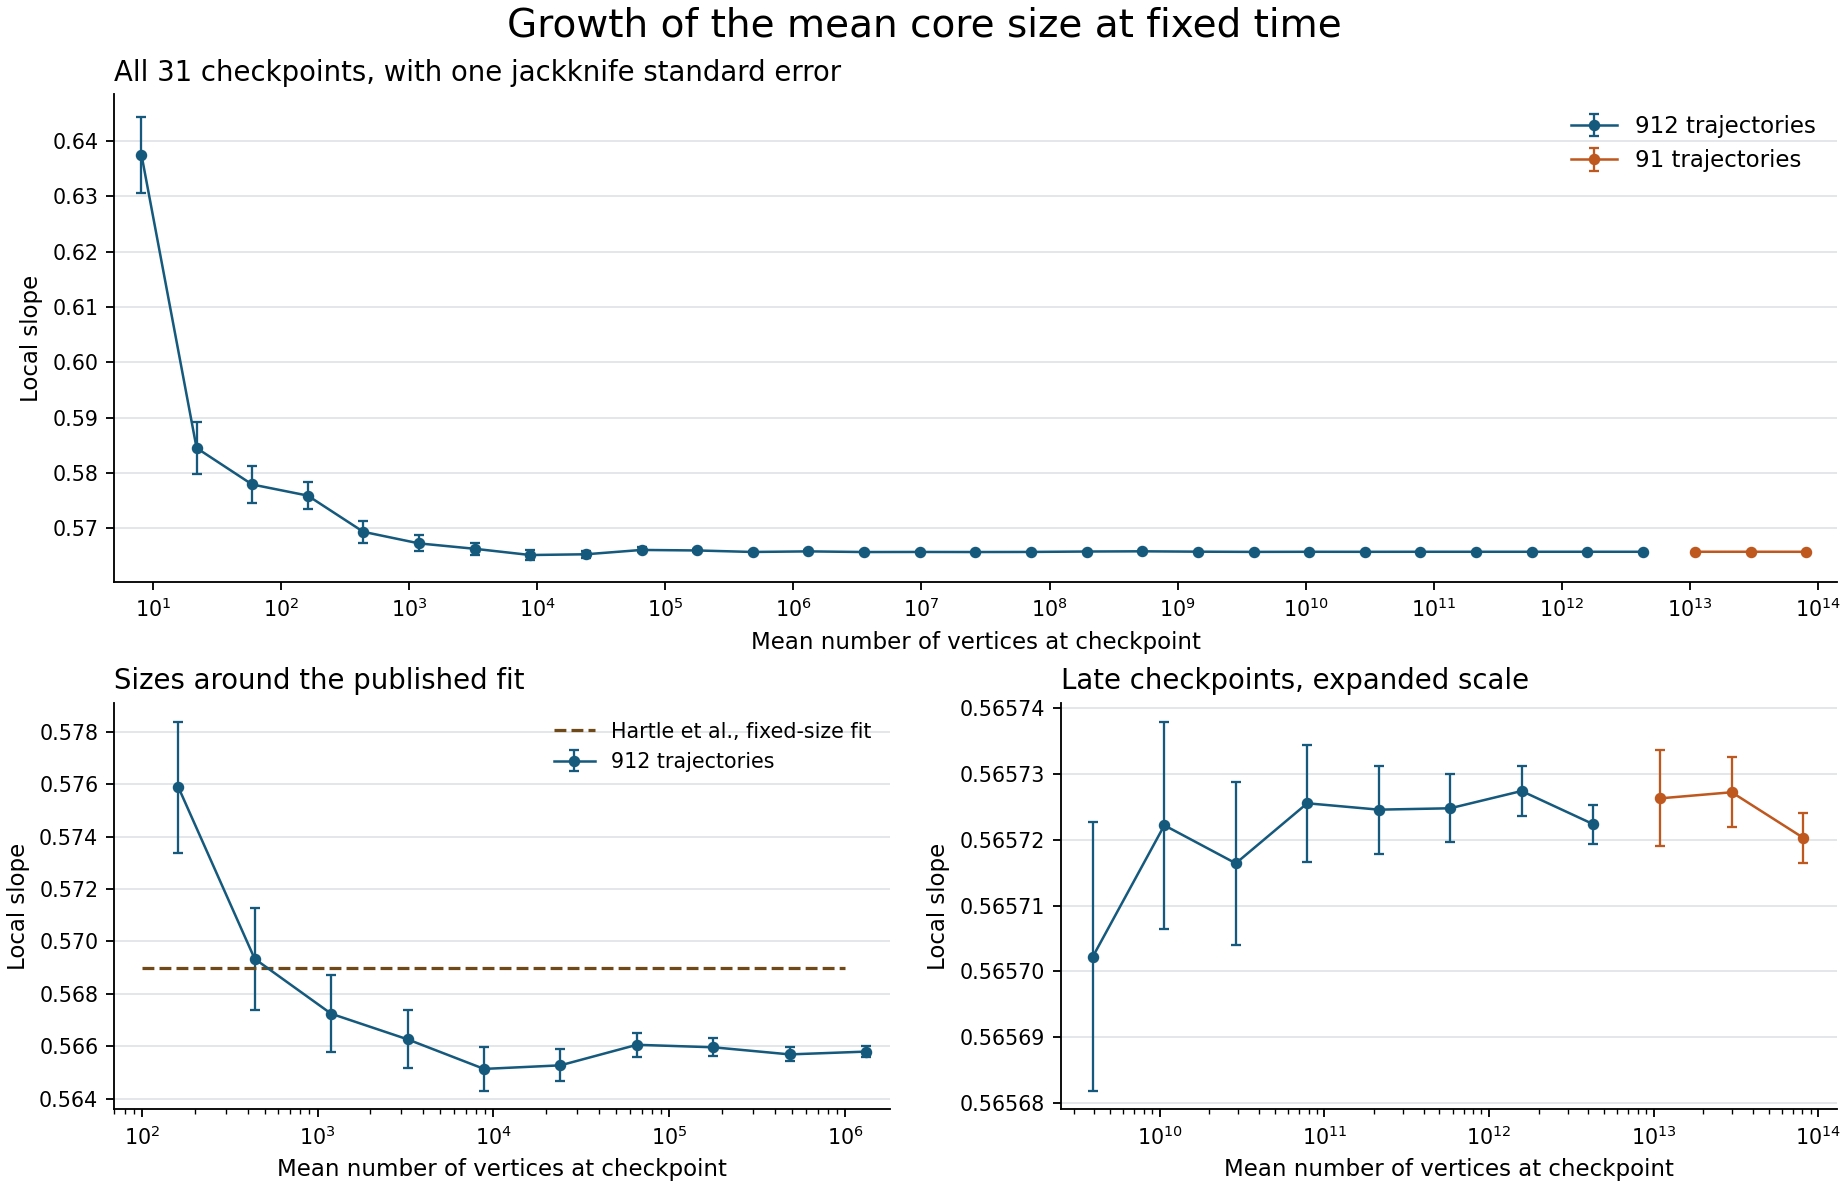
\includegraphics[width=\linewidth]{local_slopes.png}
\caption{Core growth at integer times $1$ through $31$. The horizontal
coordinate is the sampled mean population. Bars give one delete-one-trajectory
jackknife standard error. Through $t=28$ there are $912$ trajectories; $91$
continue to $t=31$. The lower panels enlarge the region around the published size range and
the late checkpoints, respectively. The dashed line marks the single
fixed-size fit of Hartle et al.\ over its fitted range.}
\label{fig:slopes}
\end{figure}

At the last checkpoint the sampled mean population is $8.117\times10^{13}$ and the estimated local
slope is $0.5657203\pm0.0000038$. A second estimate pools the pre-firing
conversion probabilities over $22{,}223{,}928{,}834$ core firings in windows
after $t=21$, dividing their sum by the number of firings. It gives
$0.5657230\pm0.0000032$; using realized conversions gives
$0.5657253\pm0.0000032$. A separate implementation, with $48$ independent
runs, gives $0.5657242\pm0.0000175$ for the instantaneous ratio at $t=27$.
These uncertainties measure sampling variation at the stated horizons.
The simulations provide no bound on the distance from these estimates to
$\mu$. The supplement includes the generators, archived trajectories for
the pooled sample, fixed-size data and scripts that reproduce the fits and
figure.

\section{Open problems}
Addario-Berry et al.\ asked about normalization and degree counts in \cite[Sec.~7, Questions~1--2]{AB}. The common logarithmic exponent resolves the exponent part of this problem. The exact value of $\mu$ is unknown. Theorems~\ref{th:exist}
and~\ref{th:bracket} leave open whether $\E C_n$ is asymptotic to a constant
times $n^\mu$, and whether $C_n/\E C_n$ converges to a positive
non-degenerate random variable. For degrees, the corresponding open
questions include a sample-path law uniform in growing $k$ and the
leading asymptotics for the exact degree counts and their dependence on $k$ proposed in \cite{KR}. A sharper
asymptotic for the cumulative degree counts would need enough control
of adjacent counts to determine their difference.

\section*{How this work was produced}
Can Uzay selected the problem, coordinated independent attempts and set the criteria for proofs and exact arithmetic. Generative AI systems in the GPT, Gemini and Claude families developed the mathematical arguments, certificates and simulation programs, drafted and revised the manuscript, and reviewed the proofs in separate sessions. Exact arithmetic checks the finite inequalities. Independent implementations, direct calculations on small trees and deliberate perturbations also tested the constructions. The supplement records the model contributions and review reports. The sole listed author is responsible for the manuscript. No human referee has yet read the proofs.

\appendix
\section{The motif drift inequalities}\label{app:motif}
\subsection{The four weight tables}

Both certificates use $D_0=24$, $K_T=12$, $L_F=800$ and $K_F=150$.
For a vertex weight use the projection
\[
 \pi(L,k,h)=
 \begin{cases}(\min(L,L_F),k,h),& k\le K_F,\\
 \star_h,&k>K_F.\end{cases}
\]
Write $f(s)$ for the value of the vertex table at $\pi(s)$.
For the other weights, retain the inner states $\mathcal I=\{s:2\le D<D_0\}$
individually. A tail state has $D\ge D_0$. Introduce the symbols $\infty$
and $q_{\kappa h}$, where $\kappa=\min(k,K_T+1)$ and $h\in\{0,1\}$.
The probability measure representing a state on these indices is
\[
 \zeta_s=
 \begin{cases}
   \delta_s,&s\in\mathcal I,\\
   (1-t)\delta_\infty+t\delta_{q_{\kappa h}},\quad t=D_0/D,
       &D\ge D_0 .
 \end{cases}
\]
At these indices put $i(s)=1/D$ for inner $s$, $i(\infty)=0$ and
$i(q_{\kappa h})=1/D_0$. Thus $\sum_a\zeta_s(a)i(a)=1/D$ exactly.
Let $\mathcal P$ consist of $\infty$ and the indices with $k\ge1$
(or $\kappa\ge1$), and let $\mathcal W$ consist of $\infty$ and the
indices with $h=1$. These are the possible parent and child indices on a
core edge. The centre domains for the three-vertex motifs are
\[
 H=\{(L,k,1):1\le k\le8,\ D<16\},\qquad
 J=\{(L,k,h):2\le k\le6,\ D<12\}.
\]

The edge table $g[a,b]$ is on $\mathcal P\times\mathcal W$, with zero
entries for two tail indices. The vertical path table $h_V[a,s,b]$ is on
$\mathcal P\times H\times\mathcal W$. The cherry table $h_C[s,b_1,b_2]$
is on $J\times\mathcal W^2$ and is symmetric in $b_1,b_2$. Extend each
three-vertex weight by zero when the centre is outside its domain. Evaluate
all endpoint arguments by averaging independently at each endpoint under its measure $\zeta_s$. For example,
\[
 g(p,w)=\sum_{a,b}\zeta_{s_p}(a)\zeta_{s_w}(b)g[a,b],\qquad
 h_V(p,u,w)=\sum_{a,b}\zeta_{s_p}(a)\zeta_{s_w}(b)h_V[a,s_u,b].
\]
Write $p\to w$ for a core edge directed away from the root and
$B(u)$ for the set of core children of $u$. The potential is
\begin{align*}
 \Phi(T)={}&\sum_{u\in K} f(s_u)+\sum_{p\to w}g(p,w)
       +\sum_{p\to u\to w}h_V(p,u,w)\\
       &+\sum_{u\in K}\ \sum_{\{w_1,w_2\}\subset B(u)}h_C(u,w_1,w_2).
\end{align*}
Each unordered pair in the last sum consists of distinct vertices.
In addition to these weights, the certificates give five numbers
$r_{\mathrm{par}},r_{\mathrm{ch}},x_{\mathrm{par}},x_{\mathrm{ch}},x_{cc}$ and three functions
$A_{pc},A_{cp},A_{cc}$ at each inner state. Each function is linear between
successive points of the common knot set
\[
  \Xi=\tfrac1{240}\{0,10,15,25,40,60,80,100,120\}.
\]
The second knot is $1/D_0$ and the last is $1/2$. The five numbers have
denominator $10^6$, and the weights and knot ordinates have denominator
$10^{10}$ before reduction.

\subsection{Decomposition of the generator}

For an existing term $\tau$ with vertex set $S(\tau)$, let $\Delta_x\tau$
and $\nabla_x\tau$ be its changes under $s_x\mapsto s_x^+$ and
$s_x\mapsto s_x^b$, respectively, with the same vertices in the term.
Put $G(\tau)=\sum_{x\in S(\tau)}(r_x\Delta_x\tau+b_x\nabla_x\tau)$.
The sum of the additional terms created by budding at $x$ is
\[
 f(\nu)+g(x^b,\nu)+h_V(p_x,x^b,\nu)
                +\sum_{w\in B(x)}h_C(x^b,w,\nu).
\]
Here $x^b$ means $x$ with its new state, and the path is omitted at the
root. The newborn has no core children, which gives exactly this list.
Entry into $H$ requires budding from $k=0$, when no old path through
that centre existed. Entry into
$J$ requires budding from $k=1$, when there was no old cherry.
Indeed $D,k$ never decrease and $h$ is fixed. Exits are included in the
jumps by the zero extension. Thus $\mathcal L\Phi$ is the sum of the
$G(\tau)$ and of the displayed newborn terms multiplied by $b_x$.

We redistribute this sum before bounding it. For an inner $u$ keep
$\theta_u=h_u r_{\mathrm{par}}(s_u)+k_u r_{\mathrm{ch}}(s_u)$ in place of $\rho_u$
in the vertex rate, and transfer each difference to the edge from which the
neighbour contribution came. For a tail $u$ keep $\theta_u=\rho_u$.
Assign the newborn vertex and edge to $u$. The resulting vertex expression is
\begin{equation}\label{eq:motif-vertex}
 V_u=(L_u+\theta_u)\Delta_u f
        +b_u\bigl(\nabla_u f+f(\nu)+g(u^b,\nu)\bigr).
\end{equation}
For $e=(p\to w)$ the transferred vertex contributions are
\[
 U_e=[s_p\in\mathcal I](i_w-r_{\mathrm{ch}}(s_p))\Delta_p f
      +[s_w\in\mathcal I](i_p-r_{\mathrm{par}}(s_w))\Delta_w f .
\]
Brackets around conditions denote indicators, and a summand with false
condition is omitted before evaluating any of its factors.

Next consider the gain jump $d=\Delta_x g(e)$ at an inner endpoint $x$
of $e$. Let $y$ be the other endpoint and $z\ne y$ another core neighbour
of $x$. The contribution $i_z d$ has three possible orientations. In the
following table, $p$ and $c$ in a subscript mean parent and child of $x$,
in the order $z,y$.
\[
\begin{array}{ccccc}
 z & y & \text{centre domain} & \text{centring value }a
                                      & \text{function outside the domain}\\ \hline
 \text{parent} & \text{child} & H & x_{\mathrm{par}} & A_{pc}\\
 \text{child} & \text{parent} & H & x_{\mathrm{ch}} & A_{cp}\\
 \text{child} & \text{child} & J & x_{cc} & A_{cc}
\end{array}
\]
All entries in the last two columns are taken at $s_x$. Inside the centre
domain keep $ad$ on $e$ and put $(i_z-a)d$ on the unique path or cherry
through $z,x,y$. Outside it keep $i_zd-A(i_z)$ on $e$ and put $A(i_z)$
on the edge joining $x$ and $z$. The contribution from $y$ itself is kept
on $e$. At a tail endpoint the entire gain rate stays on its edge.

For clarity, the following formula records the multiplicities on
$e=(p\to w)$. Set
\begin{align*}
 n_1&=[s_p\in\mathcal I\setminus H]h_p,&
 n_2&=[s_p\in\mathcal I\setminus J](k_p-1),&
 n_3&=[s_w\in\mathcal I\setminus H]k_w .
\end{align*}
Write $d_p=\Delta_p g(e)$ and $d_w=\Delta_w g(e)$.
For inner endpoints the retained rates, apart from the remainders, are
\begin{align*}
 \sigma_p&=L_p+i_w+[s_p\in H]x_{\mathrm{par}}(s_p)
                    +[s_p\in J](k_p-1)x_{cc}(s_p),\\
 \sigma_w&=L_w+i_p+[s_w\in H]k_w x_{\mathrm{ch}}(s_w).
\end{align*}
At a tail endpoint put $\sigma_x=r_x$. Denote the three functions at
state $s_x$ by $A_{pc}^x,A_{cp}^x,A_{cc}^x$. The total received from
other edges is
\begin{align*}
 I_e={}&n_3 A_{pc}^w(i_p)+n_1 A_{cp}^p(i_w)+n_2 A_{cc}^p(i_w).
\end{align*}
The table gives the terms summed in $R_e$. A row contributes only if its
multiplicity is positive.
\[
\begin{array}{ccl}
 \text{multiplicity} & \text{neighbour }z & \text{contribution per neighbour}\\ \hline
 n_1 & \text{parent of }p & i_zd_p-A_{pc}^p(i_z)\\
 n_2 & z\in B(p)\setminus\{w\} & i_zd_p-A_{cc}^p(i_z)\\
 n_3 & z\in B(w) & i_zd_w-A_{cp}^w(i_z).
\end{array}
\]
The newborn cherry involving $w$ after a bud at $p$ belongs to $e$,
as does the newborn path after a bud at $w$. Thus the edge expression is
\begin{align}
 E_e={}&U_e+I_e+R_e+\sigma_p d_p+\sigma_w d_w \nonumber\\
      &+b_p\bigl(\nabla_p g(e)+h_C(p^b,w,\nu)\bigr)
       +b_w\bigl(\nabla_w g(e)+h_V(p,w^b,\nu)\bigr).
       \label{eq:motif-edge}
\end{align}
Finally the expressions for a path through $u\in H$ and a cherry at
$u\in J$ (meaning $s_u$ lies in the indicated set) are
\begin{align}
 P_{puw}={}&G(h_V(p,u,w))+(i_p-x_{\mathrm{par}}(s_u))\Delta_u g(u,w)
                 \nonumber\\
           &\quad+(i_w-x_{\mathrm{ch}}(s_u))\Delta_u g(p,u),
                 \label{eq:motif-path}\\
 B_{u12}={}&G(h_C(u,w_1,w_2))
       +(i_{w_1}-x_{cc}(s_u))\Delta_u g(u,w_2)
                 \nonumber\\
           &\quad+(i_{w_2}-x_{cc}(s_u))\Delta_u g(u,w_1).
                 \label{eq:motif-cherry}
\end{align}
\begin{lemma}[Exact generator decomposition]\label{lem:decompose}
For every rooted tree arising from $T_3$, the scaled generator satisfies
\begin{equation}\label{eq:motif-sum}
 \mathcal L\Phi=\sum_{u}V_u+\sum_e E_e
       +\sum_{p\to u\to w:\,s_u\in H}P_{puw}
       +\sum_{u:\,s_u\in J}\ \sum_{\{w_1,w_2\}\subset B(u)}B_{u12}.
\end{equation}
\end{lemma}
\begin{proof}
The two events at each vertex either update the states in an old term or
create a term containing the newly promoted vertex. Equation~\eqref{eq:motif-vertex}
accounts for the newborn vertex and its parent edge, while
\eqref{eq:motif-edge} accounts for every new path and sibling pair.
For the gain at each old endpoint, summing its retained part and its
transferred part gives back the original neighbour credit times the jump.
Each path receives one residual from each of its two edges, and each
unordered sibling pair receives one for each order of its two children,
as in \eqref{eq:motif-path} and~\eqref{eq:motif-cherry}. This accounts once
for every contribution to the generator.
\end{proof}

\subsection{Reduction to finite inequalities}\label{sec:motif-reduction}

Use $(\lambda,\preceq,M)=(1133/2000,\le,\max)$ for the upper certificate
and $(113/200,\ge,\min)$ for the lower certificate. Thus $M$ selects the
extremum needed to bound a drift in the direction $\preceq$. For a rate
interval $I=[l,h]$, put $M_I(d)=M\{ld,hd\}$. If $r\in I$, then
$rd\preceq M_I(d)$ for either sign of $d$.

\begin{lemma}\label{lem:motif-corners}
Fix the clamped child counts and parent indicators of the tail endpoints
of an edge, path or cherry. Write $c$ for a choice of either $\infty$ or
$q_{\kappa h}$ at each such endpoint, and $\omega_c$ for the product of
the corresponding weights $1-t$ or $t$. The following rules bound
each indicated expression by the $\omega_c$-average of its corner bounds,
in the direction $\preceq$.
\begin{enumerate}
\item A function affine in each endpoint parameter separately has its
actual corner values as bounds. For a jump $d$ of this form, a factor
$r\in I$ gives the corner bound $M_I(d(c))$ for $rd$, provided $I$ is
valid throughout the chosen states.
\item For a knot function $A$, a remainder $zd-A(z)$ with $0\le z\le1/2$
has corner bound
\[
       A^*(d(c))=M_{\xi\in\Xi}\{\xi d(c)-A(\xi)\}.
\]
A received term $A(i_v)$ at a tail endpoint $v$ equals its corner average.
\item At a tail endpoint $v$ abbreviate $q=q_{\kappa h}$, and let $F$
be the motif table with the other arguments held fixed. Its own two event
contributions have zero bound at $\infty$. At $q$ their respective bounds
are
\begin{align*}
 &M_{[\gamma_0,1]}(F[\infty]-F[q]),\\
 &M_{[\beta_0,1]}(F[q_{\kappa+1,h}]-F[q])\quad(\kappa\le K_T),
\end{align*}
with zero budding contribution for $\kappa=K_T+1$. Here
$\gamma_0=(D_0-\kappa-h)/(D_0+1)$ and
$\beta_0=(D_0-\kappa-h)/D_0$ for $\kappa\le K_T$, and
$\gamma_0=0$ for $\kappa=K_T+1$.
\item Suppose a tail endpoint $v$ contributes $i_v$ to the gain rate at
another vertex $x$ of the same motif $F$. Put
$d_0=(\Delta_x F)|_{v=\infty}$ and $d_1=(\Delta_x F)|_{v=q}$.
The corner bounds for $i_v\Delta_x F$ are
\begin{equation}\label{eq:motif-quadratic}
     0\quad(v=\infty),\qquad D_0^{-1}M\{d_0,d_1\}\quad(v=q),
\end{equation}
with all other endpoint arguments set to their respective corners.
\end{enumerate}
\end{lemma}

\begin{proof}
Successive linear interpolation gives $d=\sum_c\omega_c d(c)$. For any
actual $r\in I$, bounding $r d(c)$ at each corner and taking the same
average proves the rate assertion. For fixed $d$, the expression $zd-A(z)$
is linear on each knot interval, so its extrema occur at knots. A maximum
of affine functions of $d$ is convex and a minimum is concave. Jensen's
inequality therefore bounds $A^*(d)$ in the asserted direction.
Since $[0,1/D_0]$ is the first knot interval,
$A(t/D_0)=(1-t)A(0)+tA(1/D_0)$.

At a tail endpoint, leaf gain changes $t=D_0/D$ by $-t/(D+1)$. Thus
\[
 r_v\Delta_v F=t\,\frac{r_v}{D+1}\bigl(F[\infty]-F[q]\bigr).
\]
The ratio is at most one. If $\kappa\le K_T$ it is at least
$(D-\kappa-h)/(D+1)$, which is increasing in $D$ and hence at least
$\gamma_0$. The clamped case uses $r_v\ge0$. Budding keeps $t$ fixed
and changes $q$ only for $\kappa\le K_T$, in which case its contribution
is $t b_v(F[q_{\kappa+1,h}]-F[q])$ with
$1\ge b_v=1-(\kappa+h)/D\ge\beta_0$. The factor $t$ assigns each
extremum to the $q$ corner. If there is a second tail endpoint,
interpolate the differences in that endpoint before bounding the rate.

For the last rule, the product at fixed other endpoint parameters is
\[
 i_v\Delta_x F=\frac{t}{D_0}\big((1-t)d_0+t d_1\big)
                  \preceq\frac{t}{D_0}M\{d_0,d_1\}.
\]
With a second tail parameter, $d_0,d_1$ are each affine in it. Their
maximum is convex and their minimum concave, giving the required bound
after interpolation in that parameter. In particular, when two tail
endpoints contribute to the same gain rate, apply this rule to their
two contributions separately and add.
\end{proof}

\paragraph{Vertex inequalities.}
Write $s=(L,k,h)$, $c=k+h$ and
$B_s=b_u(\nabla_u f+f(\nu)+g(u^b,\nu))$. The five cases below bound
\eqref{eq:motif-vertex} by $\lambda f(s)$.
\begin{enumerate}
\item For $D<D_0$, evaluate $(L+h r_{\mathrm{par}}+k r_{\mathrm{ch}})\Delta_u f+B_s$
exactly. Budding preserves $D$, so the newborn edge has two inner indices.
\item For $D\ge D_0$, $k\le K_F$, $L<L_F$, take both endpoints of
$[L,L+c/2]$ as coefficients of $\Delta_u f$. Evaluate $B_s$ at
the actual $t=D_0/D$, using the post-bud count $\min(k+1,K_T+1)$.
\item For $k\le K_F$ and $L=L_F$, $\Delta_u f=0$.
Check $B_s$ with $b_u=L_F/D$, actual $t=D_0/D$, and vertex value
$f(L_F-1,k+1,h)$ after budding.
\item For $k\le K_F$ and $L\ge L_F+1$, $\Delta_u f=0$ and the post-bud
vertex value is $f(L_F,k+1,h)$, interpreted through $\pi$ also when
$k=K_F$. Set $D_*=L_F+1+k+h$. The expression $B_s$ is $b$ times a
constant plus $b$ times an affine function of $t$. Check the four
corners of
\[
    (b,t)\in[(L_F+1)/D_*,1]\times[0,D_0/D_*].
\]
Indeed $L/(L+k+h)$ is nondecreasing in $L$ and $D\ge D_*$. Separate
affinity on the rectangle covers the actual pair $(L/D,D_0/D)$.
\item For $k>K_F$, both vertex jumps vanish. The post-bud endpoint has
index $q_{K_T+1,h}$ at $t=1$ and $\infty$ at $t=0$. Here
$D\ge K_F+1+h>D_0$. Check $b(f(\nu)+g(u^b,\nu))$ at the four corners
of $[0,1]\times[0,D_0/(K_F+1+h)]$ in $(b,t)$.
\end{enumerate}
In the last two cases $g(u^b,\nu)$ uses the affine interpolation in
$t$ with the post-bud child count. All five cases include both choices
of $h$ and use only states of degree at least two.

\paragraph{Edge inequalities.}
For example, let an inner parent gain while its child has degree $48$. The
child has $t=24/48=1/2$. Its credit times the parent jump is
$(d_0+d_1)/96$, with $d_0,d_1$ the two parent jumps in
\eqref{eq:motif-quadratic}. For the upper bound the average of the two
corner charges is $\max(d_0,d_1)/48$, which bounds that term even when the
jumps have opposite signs. For the lower bound use the minimum.
For all $(a,b)\in\mathcal P\times\mathcal W$, use
\eqref{eq:motif-edge} to form the following corner expression.
Budding preserves the degree of an inner index. A gain from $D_0-1$ lands
at $q_{\kappa h}$ with $t=1$. Use these successor indices for table
differences throughout. If both indices are tail indices, the edge and
all its jumps vanish since the two degrees remain at least $D_0$.
There is no vertex transfer or remainder, and neither endpoint can create
a newborn motif centred in $H$ or $J$. Its inequality is $0=0$.
For all other pairs proceed as follows.
\begin{itemize}
\item Evaluate $U_e$, $I_e$ and both inner-end budding terms at the corner,
using $i(a),i(b)$ for the credits. Keep the two newborn terms with their
post-bud centres and use their zero extensions. The received functions
are affine over the entire tail interval by Lemma~\ref{lem:motif-corners}.
\item Replace $R_e$ by
\[
 n_1(A_{pc}^p)^*(d_p)+n_2(A_{cc}^p)^*(d_p)+n_3(A_{cp}^w)^*(d_w).
\]
Evaluate each difference at the corner, omitting zero multiplicities.
\item For an inner endpoint $x$ keep $\sigma_x\Delta_x g$, omitting
$i_y$ from $\sigma_x$ if the opposite endpoint $y$ is tail. For such a
tail $y$, add its two event bounds from Lemma~\ref{lem:motif-corners}(3)
and its contribution to $i_y\Delta_x g$ from
\eqref{eq:motif-quadratic}. In particular at $a=q$ with $b$ inner the
latter is
\[
 D_0^{-1} M\{g[\infty,b^+]-g[\infty,b],\,g[q,b^+]-g[q,b]\}.
\]
At $b=q$ with $a$ inner it is
$D_0^{-1}M\{g[a^+,\infty]-g[a,\infty],g[a^+,q]-g[a,q]\}$.
At $\infty$ all three contributions of this rule are zero.
\end{itemize}
Compare the sum with $\lambda g[a,b]$ in direction $\preceq$.

\paragraph{Path and cherry inequalities.}
For a path take each $(a,s,b)\in\mathcal P\times H\times\mathcal W$.
For a cherry take each $(s,b_1,b_2)\in J\times\mathcal W^2$, with the
child pair unordered and repetitions of an index allowed. First evaluate
the two edge contributions in \eqref{eq:motif-path} or
\eqref{eq:motif-cherry} at the corner. Each product uses the degree
credit of one endpoint and an edge jump depending on the other endpoint,
so it is separately affine. Compute the remaining terms as follows.
\begin{itemize}
\item At each inner vertex $x$ of the motif use $M_{[r_0,r_0+N/2]}(\Delta_x F)$
for its gain, where $F=h_V$ or $h_C$. The table gives $r_0$ after
removing the credits of any displayed tail neighbours, and $N$ counts the
core neighbours outside the motif. Here $u$ is its centre and $i^I_v$
denotes $i_v$ for an inner endpoint and zero for a tail endpoint.
\[
\begin{array}{lcc}
 \text{position of }x & r_0 & N\\ \hline
 \text{top }p\text{ of a path}     &L_p+i_u &h_p+k_p-1\\
 \text{bottom }w\text{ of a path} &L_w+i_u &k_w\\
 \text{middle }u\text{ of a path} &L_u+i^I_p+i^I_w &k_u-1\\
 \text{child }w_j\text{ of a cherry} &L_{w_j}+i_u &k_{w_j}\\
 \text{apex }u\text{ of a cherry} &L_u+i^I_{w_1}+i^I_{w_2} &h_u+k_u-2
\end{array}
\]
Each of the $N$ outside neighbours contributes between zero and $1/2$.
Use the exact budding contribution $b_x\nabla_x F$. A centre that exits
$H$ or $J$ gives successor weight zero for either jump.
\item For each tail endpoint $v$ add its own gain and budding bounds
from Lemma~\ref{lem:motif-corners}(3). Add \eqref{eq:motif-quadratic}
with $x=u$ for the removed centre credit $i_v\Delta_u F$. This accounts
for zero, one or two tail endpoints. Two cherry children of equal table
index are distinct vertices, so each contributes once even on the
diagonal. The apex may be the root.
\end{itemize}
Compare the result with $\lambda h_V[a,s,b]$ or
$\lambda h_C[s,b_1,b_2]$. In every edge, path and cherry case, if the
corner sum is $\widehat X(c)$ and the corresponding table weight is
$\tau[c]$, the checks imply
\[
 X(T)\preceq\sum_c\omega_c\widehat X(c)
       \preceq\lambda\sum_c\omega_c\tau[c]=\lambda\tau(T).
\]
The first inequality follows summand by summand from
Lemma~\ref{lem:motif-corners}, whose rate bounds hold for every choice of
the unseen neighbours. Together with the vertex cases and
\eqref{eq:motif-sum} this proves $\mathcal L\Phi\preceq\lambda\Phi$
once the finite comparisons have been made.

\subsection{Comparison with core size and evaluation of the certificates}

Assign each edge and vertical path to its bottom vertex and each cherry to
its apex. Let $W_u$ be $f(s_u)$ plus the assigned weights, so
$\Phi=\sum_{u\in K}W_u$. The upper drift bound requires a lower bound
on $W_u$, and the lower drift bound requires an upper bound. Write $m$
for $\min$ in the former case and $\max$ in the latter. For child indices
$b$ and apex states $s\in J$ form
\begin{align*}
 g_m(b)&=m\bigl(\{0\}\cup\{g[a,b]:a\in\mathcal P\}\bigr),\\
 v_m(b)&=m\bigl(\{0\}\cup
       \{h_V[a,s',b]:a\in\mathcal P,\ s'\in H\}\bigr),\\
 c_m(s)&=m\bigl(\{0\}\cup
       \{h_C[s,b_1,b_2]:b_1,b_2\in\mathcal W\}\bigr).
\end{align*}
For an inner state put $S_u=\{s_u\}$ and for a tail state put
$S_u=\{\infty,q_{\kappa h}\}$, allowing both indices also when $t=1$.
There is at most one incoming edge and one incoming path, both absent at
the root. Their values are averages, and zero covers an absent term.
An active apex contributes precisely $\binom{k_u}{2}$ cherries.
Consequently in the upper certificate $W_u$ is at least
\[
 f(s_u)+h_u\left(m_{b\in S_u}g_m(b)+m_{b\in S_u}v_m(b)\right)
       +[s_u\in J]\binom{k_u}{2}c_m(s_u),
\]
and in the lower certificate $W_u$ is at most this expression. At the
root the parenthesis is omitted. Its extremum over all $u$ is a finite
calculation. Enumerate $0\le L\le L_F$, $0\le k\le K_F$, $h=0,1$ with
$D\ge2$, and the two overflow states $\star_h$. Increasing $L$ above
$L_F$ changes neither the projection nor $S_u$, and an overflow state is
tail with $\kappa=K_T+1$ and lies outside $J$.

\begin{lemma}\label{lem:motif-certificate}
There are rational tables giving potentials $\Phi_+,\Phi_-$ with
\begin{align*}
 \mathcal L\Phi_+&\le(1133/2000)\Phi_+,&
 \Phi_+(T)&\ge(2989767809/10^{10})\,|K|,\\
 \mathcal L\Phi_-&\ge(113/200)\Phi_-,&
 \Phi_-(T)&\le(17527873930/10^{10})\,|K|.
\end{align*}
\end{lemma}

\begin{proof}[Finite verification]
The accompanying program \texttt{cert\_build.c} produces the integer
arrays of weights and auxiliary data for each direction. Its triples
of input integers (direction, numerator, denominator) are $(1,1133,2000)$
and $(2,113,200)$. Floating-point compiler choices in this search can affect the proposed integers. The exact comparisons and constants here concern the two arrays identified below. The supplement archives lossless copies in \path{verify/motif-bracket/reference/}; decompression gives the exact inputs to the GMP checker. The reference build uses GCC 13.3.0 with \texttt{-O3 -Wall -Wextra -fopenmp} and links the math library. A rebuild with a different digest requires a fresh exact check of the signs and printed constants. These SHA-256 digests identify the two verified binaries (concatenate the two lines for each direction).
\begin{center}\small
\begin{tabular}{l@{\quad}l}
Upper & \texttt{3a4aef888a5b567a8ada05f9546f98c9}\\
      & \texttt{79d361da9f9b33ba6e794eb91fb30abe}\\
Lower & \texttt{9e966fba9aee6eae3da659b693d3bb9c}\\
      & \texttt{481c1cea66635b5218d0887f182a60d9}
\end{tabular}
\end{center}
The degree and child cutoffs give $572$ inner states,
$601$ endpoint indices, $555$ parent indices and $290$ child indices.
There are $84$ active path centres and $75$ active cherry centres.
The vertex array has $2(801)(151)+2=241904$ entries.

For these data \texttt{cert\_verify\_gmp.c} evaluates the rational
comparisons specified above. It checks the zero block of the edge table,
then enumerates the five vertex cases, the remaining parent--child pairs,
the full product $\mathcal P\times H\times\mathcal W$, and $J$ times the
unordered pairs of child indices with repetition. For example, the path
count is $555\cdot84\cdot290$, and the cherry count is
$75\cdot290\cdot291/2$. The results in each direction are
\[
\begin{array}{lrrrr}
 & f & g & h_V & h_C\\ \hline
 \text{inequalities} & 484\,138 & 160\,545 & 13\,519\,800 & 3\,164\,625\\
 \text{failed}       & 0 & 0 & 0 & 0 .
\end{array}
\]
Vertex and edge comparisons use rational arithmetic. For a path or cherry
let $D_1,D_2$ denote the endpoint corner degrees, taking $1$ at $\infty$
and $D_0$ at $q_{\kappa h}$. Multiplying the inequality by
$Q\,10^{10}\cdot 2D_1D_uD_2(D_0+1)10^6$, where $\lambda=P/Q$,
clears every denominator. The checker compares the resulting integer
sums. The search is used only to propose these integer arrays.

The extremum of the per-vertex comparison and the initial vertex entry,
in the same integer units, are
\[
\begin{array}{lrr}
 & \text{upper certificate} & \text{lower certificate}\\ \hline
 10^{10}\ \text{times the per-vertex bound} & 2\,989\,767\,809 & 17\,527\,873\,930\\
 10^{10} f(2,0,0) & 14\,606\,753\,031 & 14\,608\,704\,616 .
\end{array}
\]
The corner reduction proves the drift inequalities for all trees, and
summing the per-vertex comparisons gives the two bounds by $|K|$.
\end{proof}

\section{Construction of the degree-band certificate}\label{app:band}
\subsection{States along a growth history}

Fix an old core vertex $u$ at size $n\ge3$ and abbreviate $D=D_u$, $c=c_u$ and $L=L_u=D-c$. Conditional on the growth history
$\mathcal F_n$, multiply one-step probabilities by $n$ and call the resulting
quantities rates. Write the gain and conversion rates at $u$ as
\[
 r_u=L+\sum_{w\sim_K u}\frac{1}{D_w},
 \qquad b_u=\frac{L}{D}.
\]
At rate $r_u$ a new leaf attaches to $u$ (a gain). At rate $b_u$
the source is $u$ and a new leaf attaches to one of its leaves (a
promotion, also called a conversion). The leaf chosen by $u$ becomes a core vertex of type $(2,1)$,
with $u$ as its creator. At $u$ the pair $(D,c)$ becomes $(D,c+1)$. These events
partition all choices of attachment target and their rates sum to $n$.
At size three the sole core vertex has $(D,c)=(2,0)$ and rates $2,1$.

For $2\le D<H=2400$ we record $(D,c)$ and a sorted multiset of $c$
neighbour labels. The table gives $h_c=h_c(D)$ by band. Omitted entries
are $2$. The last column counts all finite states in the band.
\begin{center}
\begingroup\small\setlength{\tabcolsep}{3.2pt}
\begin{tabular}{@{}l rrrrrrrrrrr r@{}}
\hline
$D$ & $h_1$ & $h_2$ & $h_3$ & $h_4$ & $h_5$ & $h_6$ & $h_7$
    & $h_8$ & $h_9$ & $h_{10}$ & $h_{11}$ & States \\
\hline
$[2,16)$      &620&240&45&13&8&6&5&4&3&3&3&53\,201\,381\\
$[16,32)$     &620&150&32&10&7&5&4&4&3&3&3&23\,199\,024\\
$[32,80)$     &620&85&21&8&6&5&4&4&3&3&3&22\,401\,552\\
$[80,200)$    &620&46&14&7&5&4&4&3&3&3& &17\,550\,960\\
$[200,500)$   &620&28&10&6&5&4&4&3&3&3& &22\,446\,000\\
$[500,1000)$  &620&19&8&5&4&4&3&3&3& & &21\,291\,500\\
$[1000,2400)$ &620&12&7&5&4&4&3&3&3& & &66\,455\,200\\
\hline
\end{tabular}
\endgroup
\end{center}

A neighbour of degree $d<h_c$ is observed individually. Its label gives
$d$ and $k=\min(c_w,K_c)$, where $K_1=20$, $K_2=7$, and $K_c=5$ for
$c\ge3$. We call $k=K_c$ saturated. If $c=1$, $d\le14$ and
$2\le k\le4$, the label also describes one distinguished core neighbour
of $w$ other than $u$. This vertex is the \emph{witness}. Its label gives
its true degree and core degree $(e,j)$ for $2\le e<6$, and a single
symbol for $e\ge6$. All $1\le j\le e$ are admitted.

For $d\ge h_c$ a pooled label stores only a lower bound $b$ on $d$.
The allowed marks, in increasing order, are $h_c$, the powers of two from
$4$ onwards strictly between $h_c$ and $H$, and $H$. Encoding a known
degree or re-encoding a lower bound uses the largest allowed mark at most
that number. Of the pooled neighbours only one may retain a mark larger
than $h_c$. Keep a largest mark and reset the other pooled marks to $h_c$.
Order the individual labels lexicographically by $(d,k)$, and within each
witness type by $(e,j)$ with the symbol for $e\ge6$ last. All pooled
labels follow all individual labels. Vertex birth order breaks ties whenever
an identity must be chosen. The initial edge may be ordered arbitrarily.

\begin{lemma}[History invariant]\label{lem:banded-history}
On every realised history the recorded low degrees and unsaturated core
degrees are exact, saturated core degrees and pooled marks are valid lower
bounds, and every required witness is an identifiable vertex at distance
two with the recorded data. The updates of an old finite state and the
state of a newly promoted vertex are determined by the following rules.
\end{lemma}
\begin{proof}
Start with the empty multiset at the centre of the three-vertex tree.
Here the centre of a row means the vertex $u$ whose state is being recorded. On a gain at $u$ replace $(D,c)$ by $(D+1,c)$. Within a band keep
the multiset. At a band boundary re-encode each old entry and retain the
largest pooled mark as above. For $c=1$ the alphabet is constant, including
its witness. At $D+1=H$ drop the multiset. On a central conversion, which
requires $L>0$, pass to $(D,c+1)$, re-encode the old entries, insert the
encoding of $(2,1)$, and apply the same largest-mark rule. This also covers
$c=0$ and the case $h_{c+1}=2$, where even the fresh neighbour is pooled.
The cutoffs and core-degree caps can only decrease in these projections.
Hence an old lower bound always supplies the information required at the
new resolution.

At an individually observed neighbour, a gain replaces $d$ by $d+1$,
preserving the witness while required. At $d+1=h_c$ the entry becomes the
first pooled mark. A conversion increments $k$ up to its cap and, if the
result requires a witness, selects the newly promoted $(2,1)$ vertex.
A saturated conversion leaves the entry fixed. At an exact witness a gain
increments $e$ (giving the pooled symbol at six), and a conversion
increments $j$. Events at already pooled neighbours or pooled witnesses
leave their marks fixed because degrees never decrease.

It remains to initialise the promoted vertex's own state. It has $(D,c)=(2,1)$
and sees its creator with the creator's unchanged degree $D_u$ and new
core degree $c_u+1$. Encode that pair in the $c=1$ alphabet. If it requires
a witness, select the first entry of the creator's \emph{old} sorted
multiset. Here $1\le c_u\le3$. Each of the corresponding cutoffs is at
least six and each core-degree cap is at least five. Thus an entry of
degree below six supplies its true pair, even at degree five and cap five,
and every other entry certifies degree at least six. This selects a core
neighbour distinct from the promoted vertex. A tail creator always gives
the sole mark $H$. These updates preserve all assertions by induction.
For example, promote a leaf of the initial centre and then let the centre gain a leaf. After promotion both core vertices have $(D,c)=(2,1)$ and record the other as their only core neighbour. The gain changes the centre to $(3,1)$ and updates its recorded degree at the other vertex to three. The labels depend on the actual history, so conditional expectations below use
$\mathcal F_n$ throughout.
\end{proof}

\subsection{The generator and the two transfers}

Let $z_u$ denote the current weight at $u$ and
$\Phi_n=\sum_{u\in K}z_u$. For an old vertex let $\Delta_x^+z_u$ and
$\Delta_x^b z_u$ be its changes on a gain and a conversion at $x$.
All choices of converted leaf at $x$ give the same numerical changes
and the same newborn weight $z_{\rm new}(x)$. Let $S_u$ consist of the
individually observed neighbours of $u$, and $J_u$ of its witness if
recorded with $e<6$. Take both sets empty in the tail. Within each
$I_u=\{u\}\cup S_u\cup J_u$ these sets are disjoint by the tree property.
A gain or conversion elsewhere leaves the old weight fixed, by
Lemma~\ref{lem:banded-history}. Interchanging the sum over events with
the sum over old vertices gives the identity
\[
 n\E[\Phi_{n+1}-\Phi_n\mid\mathcal F_n]
 =\sum_{u\in K}\left[
      \sum_{x\in I_u}(r_x\Delta_x^+z_u+b_x\Delta_x^b z_u)
       +b_u z_{\rm new}(u)\right].
\]
One step can change several old weights. Each such change occurs once in
this sum, and the new weight occurs only in its creator's row.

Two tables redistribute this drift over the rows. The first contains signed
integers $g_{uw}=g(D_u,c_u;D_w,c_w)$ for ordered core edges, with missing
entries set to zero. A nonzero entry requires $D_u,D_w<H$ and
\[
 D_w<h_{c_u}(D_u),\quad c_w<K_{c_u},\qquad
 D_u<h_{c_w}(D_w),\quad c_u<K_{c_w}.
\]
Thus both endpoints can read the same entry on every history, independently
of their witnesses. In row $u$ replace the central gain difference by
$U_u=\Delta_u^+z_u+\sum_{w\sim_K u}g_{wu}$ and the gain difference at
$w\in S_u$ by $\Delta_w^+z_u-g_{uw}$. The addition $r_u g_{wu}$ in
row $u$ cancels its subtraction in row $w$ for the very same gain at $u$.
No symmetry of $g$ is required.

The second table is nonnegative, $a(u)=a(D_u,c_u)$, with zero entries off
its finite support in $D_u<H$. For each ordered edge $w$ to $u$ with
$D_w\ge T=8$, subtract $a(u)/D_w$ from row $u$ and add it to row $w$.
This is again an exact cancellation, including an edge with a tail sender.
Writing $R_u$ for the amended row, we have $\sum_u R_u=
n\E[\Phi_{n+1}-\Phi_n\mid\mathcal F_n]$, where
\begin{align*}
 R_u={}& L U_u+\sum_{w\sim_K u}
          \frac{U_u-a(u)\ind_{\{D_w\ge T\}}}{D_w}
       +b_u\bigl(\Delta_u^b z_u+z_{\rm new}(u)\bigr)\\
 &+\sum_{w\in S_u}\bigl[
       r_w(\Delta_w^+z_u-g_{uw})+b_w\Delta_w^b z_u\bigr]
   +\sum_{x\in J_u}
       (r_x\Delta_x^+z_u+b_x\Delta_x^b z_u)\\
 &+\frac{\ind_{\{D\ge T\}}}{D}\sum_{w\sim_K u}a(w).
\end{align*}

\subsection{Finite rows and the boundary condition}

The integer inputs are trial rewards $s(t)$ for the single neighbour label
$t$ of a newborn, and the two transfer tables. Use integer weight units of
$10^{-12}$. A finite row comprises terms $(v,r_-,r_+)$, consisting of an
adjusted target weight and the lower and upper bounds on its rate.
For a proposed current weight $z$, its contribution is bounded by
\[
 Q_z(v,r_-,r_+)=
 \left\lceil\max\{r_-(v-z),\ r_+(v-z)\}\right\rceil .
\]
This chooses the lower rate on a negative difference and the upper rate on
a positive one. Every bound below is conditional on the same realised
history, so the terms may be bounded separately even when their rates are dependent.

\paragraph{Central events.}
Let $z^+$ and $z^b$ be the respective successor weights of the old vertex,
with the boundary convention below, and set $V=z^++\sum_w g_{wu}$ over
its core neighbours. Include the target $V$ at rate $L$ for gains sourced
by leaves. A group of $p$ identical individual labels of degree $d$ gives
target $V-a(u)\ind_{\{d\ge T\}}$ at rate $p/d$.
A group of $p$ pooled labels of mark $b$ gives
$V-a(u)\ind_{\{b\ge T\}}$ on the interval $[0,p/b]$. Indeed every true
degree is at least $b$. If $b<T$, any unrecorded subtraction can only
decrease the drift. A conversion gives target $z^b+s(t)$ at rate $L/D$,
with $t$ determined before projecting the creator's old multiset as in
Lemma~\ref{lem:banded-history}. Omit zero-rate terms, in particular the
conversion when $c=D$.

\paragraph{Neighbour and witness events.}
Take a representative $w$ of each individually observed group. A gain at
$w$ uses the resulting weight at $u$ minus $g_{uw}$.
Conversions at $w$ and both witness events use the unadjusted successor. The following
intervals are per representative. Multiply both ends by the group
multiplicity before applying $Q_z$.
\begin{itemize}
\item For a gain at $w$ without a witness, if $k<K_c$ the interval is
\[
 [d-k+1/D,\ d-k+1/D+(k-1)/2].
\]
There are $d-k$ leaf sources, one central source of rate $1/D$ and $k-1$
other core sources of rate at most $1/2$. At saturation the interval is
$[1/D,\ d-(k+1)/2+1/D]$, since for true core degree $k'\ge k$ the upper
bound $d-k'+1/D+(k'-1)/2$ decreases with $k'$.
\item With a witness, $k$ is exact. Set $[l,h]=[1/e,1/e]$ for an
exact witness and $[l,h]=[0,1/6]$ for a pooled one. The near gain has
interval $[d-k+1/D+l,\ d-k+1/D+h+(k-2)/2]$, since only $k-2$ other
core sources remain unknown.
\item A near conversion at $k<K_c$ and $k<d$ has rate $(d-k)/d$ and
uses the successor with core degree incremented, choosing a fresh
witness if required. At $k=d$ the true rate is zero. At saturation
every possible conversion leaves the recorded label fixed.
\item An exact witness $(e,j)$ gains at a rate in
$[e-j+1/d,\ e-j+1/d+(j-1)/2]$, by counting its $e-j$ leaf sources, its
near neighbour and the other $j-1$ core sources. It converts at rate
$(e-j)/e$ when $j<e$. These events update only the witness label.
A pooled witness has no such terms.
\end{itemize}
At the sender, let $a_{\max}(t)$ be the maximum table value over true
neighbour types consistent with label $t$, including the value zero.
For an individual label fix $d$ and use its exact $k$ or all
$K_c\le k'\le d$ at saturation. For a pooled mark $b$ allow all
$d'\ge b$ and $1\le k'\le d'$. The remaining charge in $R_u$ is bounded by
\[
 F_u=\ind_{\{D\ge T\}}
     \left\lceil\frac{1}{D}\sum_t p_t a_{\max}(t)\right\rceil ,
\]
where $p_t$ is the multiplicity. Once the newborn comparisons hold, the
sufficient inequality for a finite row is therefore
\begin{equation}\label{eq:banded-row}
 F_u+\sum_{(v,r_-,r_+)}Q_z(v,r_-,r_+)
       \ \le\ \lfloor\lambda z\rfloor .
\end{equation}

\paragraph{Degrees at least $H$.}
Put $q=L/D$ and use the weight $A+Bq$ with $A>0$, $B\ge0$.
A gain increases $q$ by $(1-q)/(D+1)$ and a conversion decreases it
by $1/D$. Thus the scaled drift of $q$, summed over the
two events, is
\[
 r_u\frac{1-q}{D+1}-\frac{q}{D}\le 1-q,
 \qquad r_u\le L+c/2\le D.
\]
Here all signed transfers and $a(u)$ vanish. The sender charge is at most
$a_*c/D=a_*(1-q)$, where $a_*=\max a$. Each conversion has trial reward
$s=s(H)$. Hence the amended row, with the trial newborn, is at most
$(B+a_*)(1-q)+sq$. Both this expression and $\lambda(A+Bq)$ are affine
in $q$. Their endpoint comparisons are
\[
 B+a_*\le\lambda A,\qquad s\le\lambda(A+B).
\]
The data give $s=1000000000000$, $a_*=398437500000$,
$A=1380739398522$ and $B=383976882193$. After multiplication by $9983$
the two right sides exceed the left sides by $6235$ and $4755$.
For a finite gain from $D=H-1$ use the integer target
$A+\lceil B(L+1)/H\rceil$. Rounding this target up is valid for each
nonnegative gain rate.

\subsection{The integer recursion and its verification}

The public certificate file \texttt{recipe.txt.gz} contains the rewards
in the single-label order above (starting at index zero), the signed
entries $(D,c,d,k,g)$ and the nonnegative entries $(D,c,a)$. It has
$12\,697$ rewards, $63\,309$ signed entries and $18$ nonnegative entries.
The SHA-256 digest of the compressed input, on two consecutive lines, is
\begin{center}\small\ttfamily
584bb93c2797138ae3de54cb85c7d8e4\\
87bb7d7cc5320c021b5a64ec0cf0f60a
\end{center}

\begin{lemma}[Finite certificate]\label{lem:banded-certificate}
There are positive integer weights on all finite states satisfying
\eqref{eq:banded-row} for the given trial rewards. The completed weights
of all newborns are bounded by their trial rewards. Together with the
tail they have minimum $m=3908512529$ and initial weight
$z_{(2,0)}=1539738114735$.
\end{lemma}
\begin{proof}[Computer-assisted proof]
For each $D=H-1,\ldots,2$ and, within that degree, for
$c=D,\ldots,0$, enumerate the sorted multisets of length $c$ in reverse
lexicographic order. Admit every individual label, every multiplicity of
the first pooled mark, and at most one entry above that mark. In
particular $c=0$ contributes one empty multiset for each degree. This
enumerates a superset of the states in Lemma~\ref{lem:banded-history}.

All old target weights are available at the time of use. Central gains
increase $D$, and central conversions increase $c$ at fixed $D$. Within
one layer a near gain increases the degree or enters the first pooled
mark, a near conversion increases the unsaturated core degree, and a far
move increases the witness label. Even if a conversion replaces the
witness by $(2,1)$, its near core degree has increased. Replacing one
entry by a strictly larger one strictly advances the sorted multiset.
Entry into the pool creates only the first mark, so it cannot demote a
larger mark elsewhere. Whole-multiset projections occur only on central
moves. The sole remaining dependency, the weight at $(2,1)$ at a birth,
has already been replaced by its tabulated trial reward.

For clarity, the acceptance test for each row can be written with integers
only. Express the endpoints of each interval over a common positive
denominator $h$, as $i/h,j/h$. Start the residual at
$\lfloor5657z/9983\rfloor-F_u$ and, for each term, subtract
\[
 \left\lceil\frac{(v-z)k}{h}\right\rceil,\qquad
 k=\begin{cases}i,& v<z,\\j,&v\ge z.\end{cases}
\]
Store $z$ only if $z>0$ and the residual is nonnegative. With targets
fixed the residual is nondecreasing in $z$. A numerical proposal for $z$
therefore suffices to start the search, and its accuracy plays no part in
acceptance. After the last row, read the actual weight $z(2,1;t)$ for
every newborn label and take the minimum of $s(t)-z(2,1;t)$, including
$t=H$. This last comparison closes the recursion.

Replaying these operations in \texttt{check.cpp} gives the band counts
above and yields
\[
\begin{array}{lr}
 \text{finite rows} & 226\,545\,617\\
 \text{minimum residual in a finite row} & 3\\
 \min_t\{s(t)-z(2,1;t)\} & 4\,340\,525\\
 \text{global lower and upper weight bounds}
     & [3\,908\,512\,529,\ 1\,764\,716\,280\,715]\\
 \text{weight at $(2,0)$} & 1\,539\,738\,114\,735 .
\end{array}
\]
An independent implementation, \texttt{verify\_banded.cpp}, chooses the
least admissible positive integer in each row. On the same input it
checks all $226\,545\,617$ rows, with minimum residual zero and minimum
newborn reserve $4\,341\,454$. Its initial weight and global minimum are
$1539738113358$ and $3908512428$, respectively. The first construction
gives the constants stated in the lemma.
\end{proof}

\begin{thebibliography}{99}
\raggedright
\bibitem{SK} J.~Saramäki and K.~Kaski, Scale-free networks generated by random
walkers, \emph{Physica A} \textbf{341} (2004), 80--86.
\href{https://doi.org/10.1016/j.physa.2004.04.110}{doi:10.1016/j.physa.2004.04.110}. \href{https://arxiv.org/abs/cond-mat/0404088}{arXiv:cond-mat/0404088}.
\bibitem{ES} T.~S.~Evans and J.~P.~Saramäki, Scale-free networks from self-organization, \emph{Physical Review E} \textbf{72} (2005), 026138. \href{https://doi.org/10.1103/PhysRevE.72.026138}{doi:10.1103/PhysRevE.72.026138}.
\bibitem{HIH} M.~K.~Hassan, L.~Islam and S.~A.~Haque, Degree distribution, rank-size distribution, and leadership persistence in mediation-driven attachment networks, \emph{Physica A} \textbf{469} (2017), 23--30. \href{https://doi.org/10.1016/j.physa.2016.11.001}{doi:10.1016/j.physa.2016.11.001}.
\bibitem{LSS} W.~Levens, A.~Szorkovszky and D.~J.~T.~Sumpter,
Friend of a friend models of network growth, \emph{Royal Society Open Science}
\textbf{9} (2022), 221200. \href{https://doi.org/10.1098/rsos.221200}{doi:10.1098/rsos.221200}.
\bibitem{CJ} C.~Cannings and J.~Jordan, Random walk attachment graphs,
\emph{Electronic Communications in Probability} \textbf{18} (2013),
paper 77, 1--5. \href{https://doi.org/10.1214/ECP.v18-2518}{doi:10.1214/ECP.v18-2518}.
\bibitem{KR} P.~L.~Krapivsky and S.~Redner, Emergent network modularity,
\emph{Journal of Statistical Mechanics: Theory and Experiment} (2017),
073405. \href{https://doi.org/10.1088/1742-5468/aa7a3f}{doi:10.1088/1742-5468/aa7a3f}. \href{https://arxiv.org/abs/1706.01514}{arXiv:1706.01514}.
\bibitem{GKR} A.~Gabel, P.~L.~Krapivsky and S.~Redner, Highly dispersed networks by enhanced redirection, \emph{Physical Review E} \textbf{88} (2013), 050802. \href{https://doi.org/10.1103/PhysRevE.88.050802}{doi:10.1103/PhysRevE.88.050802}.
\bibitem{KRancestor} P.~L.~Krapivsky and S.~Redner, Organization of growing random networks, \emph{Physical Review E} \textbf{63} (2001), 066123. \href{https://doi.org/10.1103/PhysRevE.63.066123}{doi:10.1103/PhysRevE.63.066123}.
\bibitem{KRsurvey} P.~L.~Krapivsky and S.~Redner, The magic of networks grown by redirection, \emph{Indian Journal of Physics} \textbf{98} (2024), 3777--3787. \href{https://doi.org/10.1007/s12648-023-02874-x}{doi:10.1007/s12648-023-02874-x}.
\bibitem{Strogatz} S.~Strogatz, post on the exponent in isotropic
redirection, 20 September 2022.
\url{https://x.com/stevenstrogatz/status/1572287647715934210}.
\bibitem{AB} L.~Addario-Berry, S.~Briend, L.~Devroye, S.~Donderwinkel,
C.~Kerriou and G.~Lugosi, Random friend trees, \emph{Random Structures \& Algorithms} \textbf{69} (2026), e70082. \href{https://doi.org/10.1002/rsa.70082}{doi:10.1002/rsa.70082}.
\href{https://arxiv.org/abs/2403.20185}{arXiv:2403.20185}.
\bibitem{HKRZ} H.~Hartle, P.~L.~Krapivsky, S.~Redner and Y.~Zhang,
Anomalous scaling in redirection networks, \emph{Physical Review E}
\textbf{114} (2026), 034314.
\href{https://doi.org/10.1103/9lmp-pydp}{doi:10.1103/9lmp-pydp}. \href{https://arxiv.org/abs/2604.01540}{arXiv:2604.01540}.
\bibitem{supplement} C.~Uzay, \emph{Growth of the non-leaf population in the
random friend tree}, supplementary proofs, certificate verifiers and
simulation data. \href{https://github.com/uzay-eth/friend-tree-exponent/tree/bb536bc6b4ff7a6e085ce817c65fb85f54a9f1d4}{Supplementary material, revision \texttt{bb536bc6b4ff}}.
\end{thebibliography}
\end{document}
